% example for dissertation.sty
\documentclass[
  % Replace oneside by twoside if you are printing your thesis on both sides
  % of the paper, leave as is for single sided prints or for viewing on screen.
  oneside,
  %twoside,
  11pt, a4paper,
  footinclude=true,
  headinclude=true,
  cleardoublepage=empty
]{scrbook}

\usepackage{dissertation}
\usepackage{verbatim}
\usepackage{minted}
\usepackage[flushleft]{threeparttable} % http://ctan.org/pkg/threeparttable
\usepackage{booktabs,caption}

\setminted[c++]{ %
    linenos=true,             % Line numbers
    autogobble=true,          % Automatically remove common whitespace
    %bgcolor=dark-bg,
    frame=lines,
    framesep=2mm,
    fontsize=\footnotesize
}

\newenvironment{code}{%
    \VerbatimEnvironment
    \begin{figure}[thp]%
    \centering
    \begin{minipage}{0.8\textwidth}%
        \begin{minted}{c++}}
{%
        \end{minted}
    \end{minipage}
    \end{figure}}

% ACRONYMS -----------------------------------------------------

%import the necessary package with some options
\usepackage[acronym,nonumberlist]{glossaries}

%enable the following to avoid links from the acronym usage to the list
%\glsdisablehyper

%displays the first use of an acronym in italic
%\defglsdisplayfirst[\acronymtype]{\emph{#1#4}}

%the style of the Glossary
%\glossarystyle{listgroup}

% set the name for the acronym entries page
%\renewcommand{\glossaryname}{acronyms}

%this shall be the last thing in the acronym configuration!!
\makeglossaries

% here are the acronym entries

% these could go in an acronyms.tex file, and loaded with:
% here are the acronym entries
\newacronym{mg}{MG}{Metagenomics}
\newacronym{mt}{MT}{Metatranscriptomics}
\newacronym{mp}{MP}{Metaproteomics}
\newacronym{imp}{IMP}{Integrated Meta-omic Pipeline}
\newacronym{fmap}{FMAP}{Functional Mapping and Analysis Pipeline}
\newacronym{ngs}{NGS}{Next Generation Sequencing}
\newacronym{solid}{SOLiD}{Sequencing by Oligo Ligation Detection}
\newacronym{pcr}{PCR}{Polymerase Chain Reaction}
\newacronym{kb}{Kb}{Kylobase}
\newacronym{mb}{Mb}{Megabase}
\newacronym{gb}{Gb}{Gygabase}
\newacronym{tb}{Tb}{Terabase}
\newacronym{smrt}{SMRT}{Single Molecule Real Time}
\newacronym{gc}{GC}{Guanine/Cytosine}
\newacronym{bp}{bp}{Base Pair}
\newacronym{cds}{CDS}{Coding Sequence}
\newacronym{ebi}{EBI}{European Bioinformatics Institute}
\newacronym{ko}{KO}{KEGG Orthologous}
\newacronym{kfu}{KFU}{KEGG Filtered UniProt}
\newacronym{mpa}{MPA}{Meta Proteome Analyzer}
\newacronym{uniprot}{UniProt}{Universal Protein Resource}
\newacronym{kegg}{KEGG}{Kyoto Encyclopedia of Genes and Genomes}
\newacronym{cdd}{CDD}{Conserved Domains Database}
\newacronym{ncbi}{NCBI}{National Center for Biotechnology Information}
\newacronym{pir}{PIR}{Protein Information Resource}
\newacronym{sib}{SIB}{Swiss Institute of Bioinformatics}
\newacronym{otu}{OTU}{Operational Taxonomic Unit}
\newacronym{orf}{ORF}{Open Reading Frame}
\newacronym{ms}{MS}{Mass Spectrometry}
\newacronym{hmm}{HMM}{Hidden Markov Models}
\newacronym{mosca}{MOSCA}{Meta-Omics Software for Community Analysis}
\newacronym{dna}{DNA}{Deoxyribonucleic acid}
\newacronym{de}{DE}{Differential Expression}
\newacronym{rrna}{rRNA}{Ribossomal RNA}
\newacronym{rna}{RNA}{Ribonucleic acid}
\newacronym{mrna}{mRNA}{Messenger RNA}
\newacronym{snp}{SNP}{Single nucleotide polymorphism}
\newacronym{nr}{NR}{Non redundant}
\newacronym{se}{SE}{Single end}
\newacronym{pe}{PE}{Paired end}
\newacronym{tpm}{TPM}{Transcripts per million}
\newacronym{dsdna}{dsDNA}{double stranded DNA}
\newacronym{cdna}{cDNA}{complementary DNA}
\newacronym{rpkm}{RPKM}{Reads Per Kilobase per Million}
\newacronym{embl-ebi}{EMBL-EBI}{European Bioinformatics Institute}
\newacronym{rpk}{RPK}{Reads per kilobase}
\newacronym{mm}{MM}{Meta-metabolomics}
\newacronym{hplc}{HPLC}{High Performance Liquid Chromatography}
\newacronym{gui}{GUI}{Graphical User Interface}
\newacronym{lcfa}{LCFA}{long-chain fatty acids}
\newacronym{blast}{BLAST}{Basic Local Alignment Search Tool}
\newacronym{api}{API}{Application Programming Interface}
% when using this, you may want to remove 'nomain' from the package options
%% **MORE INFO** %%

%to add the acronyms list add the following where you want to print it:
%\printglossary[type=\acronymtype]
%\clearpage
%\thispagestyle{empty}

%to use an acronym:
%\gls{qps}

% compile the thesis in command line with the following command sequence:
% pdlatex dissertation.tex
% makeglossaries dissertation
% bibtex dissertation
% pdlatex dissertation.tex
% pdlatex dissertation.tex

% ----------------------------------------------------------------

% Title
\titleA{Development of an automated pipeline}
\titleB{for meta-omics data analysis}

% Author
\author{Jo\~{a}o Carlos Sequeira da Costa}

% Supervisor(s)
\supervisor{Andreia Filipa Ferreira Salvador}
\cosupervisor{Miguel Francisco Almeida Pereira Rocha}

% University (uncomment if you need to change default values)
% \def\school{Escola de Engenharia}
% \def\department{Departamento de Inform\'{a}tica}
% \def\university{Universidade do Minho}
% \def\masterdegree{Computer Science}

% Date
\date{October, 2017} % change to text if date is not today

% Keywords
%\keywords{master thesis}

% Glossaries & Acronyms
%\makeglossaries  %  either use this ...
%\makeindex	   % ... or this

% Define Acronyms
%% here are the acronym entries
\newacronym{mg}{MG}{Metagenomics}
\newacronym{mt}{MT}{Metatranscriptomics}
\newacronym{mp}{MP}{Metaproteomics}
\newacronym{imp}{IMP}{Integrated Meta-omic Pipeline}
\newacronym{fmap}{FMAP}{Functional Mapping and Analysis Pipeline}
\newacronym{ngs}{NGS}{Next Generation Sequencing}
\newacronym{solid}{SOLiD}{Sequencing by Oligo Ligation Detection}
\newacronym{pcr}{PCR}{Polymerase Chain Reaction}
\newacronym{kb}{Kb}{Kylobase}
\newacronym{mb}{Mb}{Megabase}
\newacronym{gb}{Gb}{Gygabase}
\newacronym{tb}{Tb}{Terabase}
\newacronym{smrt}{SMRT}{Single Molecule Real Time}
\newacronym{gc}{GC}{Guanine/Cytosine}
\newacronym{bp}{bp}{Base Pair}
\newacronym{cds}{CDS}{Coding Sequence}
\newacronym{ebi}{EBI}{European Bioinformatics Institute}
\newacronym{ko}{KO}{KEGG Orthologous}
\newacronym{kfu}{KFU}{KEGG Filtered UniProt}
\newacronym{mpa}{MPA}{Meta Proteome Analyzer}
\newacronym{uniprot}{UniProt}{Universal Protein Resource}
\newacronym{kegg}{KEGG}{Kyoto Encyclopedia of Genes and Genomes}
\newacronym{cdd}{CDD}{Conserved Domains Database}
\newacronym{ncbi}{NCBI}{National Center for Biotechnology Information}
\newacronym{pir}{PIR}{Protein Information Resource}
\newacronym{sib}{SIB}{Swiss Institute of Bioinformatics}
\newacronym{otu}{OTU}{Operational Taxonomic Unit}
\newacronym{orf}{ORF}{Open Reading Frame}
\newacronym{ms}{MS}{Mass Spectrometry}
\newacronym{hmm}{HMM}{Hidden Markov Models}
\newacronym{mosca}{MOSCA}{Meta-Omics Software for Community Analysis}
\newacronym{dna}{DNA}{Deoxyribonucleic acid}
\newacronym{de}{DE}{Differential Expression}
\newacronym{rrna}{rRNA}{Ribossomal RNA}
\newacronym{rna}{RNA}{Ribonucleic acid}
\newacronym{mrna}{mRNA}{Messenger RNA}
\newacronym{snp}{SNP}{Single nucleotide polymorphism}
\newacronym{nr}{NR}{Non redundant}
\newacronym{se}{SE}{Single end}
\newacronym{pe}{PE}{Paired end}
\newacronym{tpm}{TPM}{Transcripts per million}
\newacronym{dsdna}{dsDNA}{double stranded DNA}
\newacronym{cdna}{cDNA}{complementary DNA}
\newacronym{rpkm}{RPKM}{Reads Per Kilobase per Million}
\newacronym{embl-ebi}{EMBL-EBI}{European Bioinformatics Institute}
\newacronym{rpk}{RPK}{Reads per kilobase}
\newacronym{mm}{MM}{Meta-metabolomics}
\newacronym{hplc}{HPLC}{High Performance Liquid Chromatography}
\newacronym{gui}{GUI}{Graphical User Interface}
\newacronym{lcfa}{LCFA}{long-chain fatty acids}
\newacronym{blast}{BLAST}{Basic Local Alignment Search Tool}
\newacronym{api}{API}{Application Programming Interface}
\glsaddall[types={\acronymtype}]



\ummetadata % add metadata to the document (author, publisher, ...)

\begin{document}
	% Cover page ---------------------------------------
	\umfrontcover	
	\umtitlepage	
	
	\chapter*{Agradecimentos}
	
	Ao fazer esta tese, pude contar com o apoio de v\'{a}rias pessoas sem as quais este trabalho seria apenas uma sombra do que se tornou. Este \'{e} o meu obrigado a quem em mim acreditou.

    \`{A} Andreia, pois sem uma boa orientadora muito dificilmente se faz uma boa tese. Tanta corre\c{c}\~{a}o foi sempre bem aplicada, se n\~{a}o pela minha falta de conhecimento, pelo menos pela minha teimosa desaten\c{c}\~{a}o. A uma orientadora exigente at\'{e} \`{a} \'{u}ltima mensagem, que nunca deixou de acreditar em mim, o meu obrigado.
    
    Ao professor Miguel, mentor dispon\'{\i}vel para todos os momentos em que se requeria a sua aten\c{c}\~{a}o. A um excelente professor, o meu obrigado.
    
    Ao V\'{\i}tor, que quando eu estava a um passo da solu\c{c}\~{a}o, ajudou-me a resolver problema atr\'{a}s de problema. A um bom amigo, o meu obrigado.
    
    \`{A} minha Catarina, parceira nas alturas entusiasmantes, em que tudo corria bem, e nas complicadas, em que tudo era desafio. A ti, que aturaste tudo o que em mim havia a aturar, e que tamb\'{e}m nunca perdeste a tua confian\c{c}a em mim, o meu obrigado.
    
    Porque quando o trabalho aperta a fam\'{\i}lia costuma ser a primeira a ficar \`{a} dist\^{a}ncia, aos meus pais, que para tudo se prontificaram para ver o seu filho dar o \'{u}ltimo passo rumo a mestre. A quem devo tudo, o meu obrigado.
    
    E a Deus. Porque me mostras o caminho.

	% Add abstracts (en,pt) ---------------------------
	\chapter*{Abstract}
	Knowing what lies around us has been a goal for many decades now, and the new advances in sequencing technologies and in meta-omics approaches have permitted to start answering some of the main questions of microbiology - what is there, and what is it doing? The exponential growth of omics studies has been answered by the development of some bioinformatic tools capable of handling \gls{mg} analysis, with a scarce few integrating such analysis with \gls{mt} or \gls{mp} studies. Furthermore, the existing tools for meta-omics analysis are usually not user friendly, usually limited to command-line usage.

    Because of the variety in meta-omics approaches, a standard workflow is not possible, but some routines exist, which may be implemented in a single tool, thereby facilitating the work of laboratory professionals. In the framework of this master thesis, a pipeline for integrative \gls{mg} and \gls{mt} data analysis was developed. This pipeline aims to retrieve comprehensive comparative gene/transcript expression results obtained from different biological samples. The user can access the data at the end of each step and summaries containing several parameters of evaluation of the previous step, and final graphical representations, like Krona plots and \gls{de} heatmaps. Several quality reports are also generated. The pipeline was constructed with tools tested and validated for meta-omics data analysis. Selected tools include FastQC, Trimmomatic and SortMeRNA for preprocessing, MetaSPAdes and Megahit for assembly, MetaQUAST and Bowtie2 for reporting on the quality of the assembly, FragGeneScan and DIAMOND for annotation and DeSEQ2 for \gls{de} analysis.
    
    Firstly, the tools were tested separately and then integrated in several python wrappers to construct the software \gls{mosca}. \gls{mosca} performs preprocessing of \gls{mg} and \gls{mt} reads, assembly of the reads, annotation of the assembled contigs, and a final data analysis. 
    
    Real datasets were used to test the capabilities of the tool. Since different types of files can be obtained along the workflow, it is possible to perform further analyses to obtain additional information and/or additional data representations, such as metabolic pathway mapping. 
    
	\cleardoublepage
	\chapter*{Resumo}
	
	O objectivo da microbiologia, e em particular daqueles que se dedicam ao estudo de comunidades microbianas, \'{e} descobrir o que comp\H{o}e as comunidades, e a fun\c{c}\H{a}o de cada microrganismo no seio da comunidade. Gra\c{c}as aos avan\c{c}os nas t\'{e}cnicas de sequencia\c{c}\H{a}o, em particular no desenvolvimento de tecnologias de \textit{Next Generation Sequencing}, surgiram abordagens de meta-\'{o}micas que t\^{e}m vindo a ajudar a responder a estas quest\H{o}es. V\'{a}rias ferramentas foram desenvolvidas para lidar com estas quest\H{o}es, nomeadamente lidando com dados de Metagen\'{o}mica (MG), e algumas poucas integrando esse tipo de an\'{a}lise com estudos de Metatranscript\'{o}mica (MT) e Metaprote\'{o}mica (MP). Al\'{e}m da escassez de ferramentas bioinform\'{a}ticas, as que j\'{a} existem n\H{a}o costumam ser facilmente manipul\'{a}veis por utilizadores com pouca experi\^{e}ncia em inform\'{a}tica, e est\H{a}o frequentemente limitadas a uso por linha de comando.
	
	Um formato geral para uma ferramenta de an\'{a}lise meta-\'{o}mica n\H{a}o \'{e} poss\'{i}vel devido \`{a} grande variedade de aplica\c{c}\H{o}es. No entanto, certas aplica\c{c}\H{o}es possuem certas rotinas, que s\H{a}o pass\'{i}veis de serem implementadas numa ferramenta, facilitando assim o trabalho dos profissionais de laborat\'{o}rio. Nesta tese, uma pipeline integrada para an\'{a}lise de dados de MG e MT foi desenvolvida, pretendendo determinar a express\H{a}o de genes/transcriptos entre diferentes amostras biol\'{o}gicas. O utilizador tem dispon\'{i}veis os resultados de cada passo, sum\'{a}rios com v\'{a}rios par\^{a}metros para avalia\c{c}\H{a}o do procedimento, e representa\c{c}\H{o}es gr\'{a}ficas como gr\'{a}ficos Krona e heatmaps de express\~{a}o diferencial. V\'{a}rios relat\'{o}rios sobre a qualidade dos resultados obtidos tamb\'{e}m s\~{a}o gerados. A ferramenta foi constru\'{i}da baseada em ferramentas e procedimentos testados e validados com an\'{a}lise de dados de meta-\'{o}mica. Essas ferramentas s\~{a}o FastQC, Trimmomatic e SortMeRNA para pr\'{e}-processamento, Megahit e MetaSPAdes para assemblagem, MetaQUAST e Bowtie2 para controlo da qualidade dos contigs obtidos na assemblagem, FragGeneScan e DIAMOND para anota\c{c}\~{a}o e DeSEQ2 para an\'{a}lise de express\~{a}o diferencial.
	
	As ferramentas foram testadas uma a uma, e depois integradas em diferentes wrappers de python para comp\^{o}r a \glsfirst{mosca}. A \gls{mosca} executa pr\'{e}-processamento de reads de MG e MT, assemblagem das reads, anota\c{c}\H{a}o dos contigs assemblados, e uma an\'{a}lise de dados final
	
	Foram usados dados reais para testar as capacidades da \gls{mosca}. Como podem ser obtidos diferentes tipos de ficheiros ao longo da execu\c{c}\~{a}o da \gls{mosca}, \'{e} poss\'{\i}vel levar a cabo an\'{a}lises posteriores para obter informa\c{c}\~{a}o adicional e/ou representa\c{c}\~{o}es de dados adicionais, como mapeamento de vias metab\'{o}licas.

	
	% Summary Lists ------------------------------------
	\tableofcontents
	\listoffigures
	\listoftables
	%\lstlistoflistings
	\printglossary[type=\acronymtype]
	\printglossaries
	\clearpage
	\thispagestyle{empty}
	
	\pagenumbering{arabic}	
	% CHAPTER - Introduction -------------------------
	\chapter{Introduction}
	
	\section{Context and motivation}
    
    \glsfirst{ngs} technologies have evolved rapidly during the last years, generating a large amount of sequencing data obtained from a large variety of organisms. \glsfirst{mg}, \glsfirst{mt} and \glsfirst{mp} refer to the study of the genome, transcriptome and proteome of more than one organism occurring in a biological sample, respectively. In nature, microorganisms rarely occur isolated and their metabolism depends on relationships that can be established with the environment (other microorganisms, plants and animals, organic and inorganic materials). 
    
    The microbiology of several biotechnological processes is still poorly described due to the difficulty on studying complex microbial communities. This knowledge is crucial for the optimization of biotechnological processes which depend on the activity and interaction of highly diverse microbial communities.
    
    The bioinformatics tools utilized for the study of an isolated organism are usually not suitable for the analysis of diverse communities. Tools for studying complex microbial systems are usually in house developed tools, non-available for the scientific community. There are also freely available tools but usually require deep knowledge on bioinformatics, which most biologists and engineers don't have. Also, some existing tools are not flexible because they were created to address specific questions and to deal with specific data formats.
    
    More recently, open-source pipelines for analyzing meta-omics data have been developed, and several advantages, but also drawbacks can be pointed out. One of the major limitations of both \gls{mp} and \gls{mt}, but also \gls{mg} analysis, is the difficulty in choosing the reference database for mapping and identifying the expressed genes and proteins. Using \gls{mg} data as a reference to identify transcripts and proteins can greatly increase the identification rates \citep{heyer2017challenges}. In order to further increase the number of genes/proteins identified, \textit{de novo} options, such as assembling without a reference, or aligning nucleotidic reads against more general databases, can be considered, which do not rely only in reference-based approaches and are particularly relevant in the analysis of complex microbial communities which are poorly characterized. \gls{imp} \citep{Narayanasamy2016} and \gls{fmap} \citep{Kim2016} already consider some of these aspects. These and other pipelines were reviewed and compared with the pipeline developed in the framework of this thesis, \glsfirst{mosca}.
    
    For the various tasks of meta-omics analysis, several tools were tested in their direct, command line interface, and then integrated in python wrappers. Several options exist for every task at hand, but only one tool was chosen for every task, with the exception of the assemblers, because of the reported difference between MetaSPAdes and Megahit results \citep{Vollmers2017}, and the databases for annotation, since different biological databases may contain profoundly different information available for the same sequences. The end goal is always to provide files in useful formats for posterior handling, and the output files from each step are made available.
    
    Testing the tool with \gls{dna} and \gls{rna} samples collected from anaerobic bioreactors, containing both \gls{mg} and \gls{mt} information, allowed for a comprehensive application of the entirety of the workflow.

    \section{Objectives and plan}

    The objective of this thesis was to develop an easy-to-use bioinformatics pipeline for integrated \gls{mg} and \gls{mt} data analysis, allowing the comparative analysis between different samples.
    
    To attain this global objective, the following specific aims were defined:
    \begin{enumerate}
        \item To review state-of-the-art pipelines for meta-omic analysis, identifying their advantages and disadvantages, and the tools integrated in their workflows.
        \item To create a mostly automated pipeline by only requiring the user input at the beginning to give general information on the type of the data, the place where the data is stored, the assembler to use in the assembly step and the database for the annotation step.
        \item To integrate and adapt selected tools which can improve data analysis and comparison, and define and construct workflows for different types of analyses.
        \item To test selected tools with real datasets, obtained from anaerobic digesters from the host research group.
    \end{enumerate}
    
    \section{Thesis organization}
    
    This thesis presents the construction of \gls{mosca}, and the reasoning behind its build up and necessity. Chapter 2 exposes the fields of \gls{mg} and \gls{mt}, their possibilities and challenges. It exposes the major steps in the bioinformatic workflow necessary to obtain meaningful information from the datasets produced in the laboratory, and presents several tools designed for tackling the challenges of the several phases of meta-omics analysis. Several pipelines which integrate these tools into a single software are also explored and the implemented tools and approaches identified.
    
    Chapter 3 explains how \gls{mosca} was designed, the reasoning behind the choice of the tools and how they were tested and integrated. The entire picture of tools, functionalities and input/output files is presented in this chapter.
    
    In chapter 4, the results obtained with real datasets, for testing the pipeline, are shown.
    
    Chapter 5 closes the thesis with the final remarks concerning \gls{mosca} in its present form, and future prospects. 

	% CHAPTER - State of the Art ---------------------
	\chapter{State of the art}
    
	\section{Overview of Next Generation Sequencing technologies}
	
	In 1977, two \gls{dna} sequencing techniques were developed, by Frederick Sanger and Walter Gilbert, based on the chain-termination method and chemical modification of \gls{dna} respectively. The first generation of sequencing techniques was dominated by Sanger's approach, even though it presented laborious work, used radioactive chemicals, was expensive and slow. This technique went on as the main solution to \gls{dna} sequencing until the end of the Human Genome Project. 
	
	Even though sequencing is the best tool for comprehensive analysis of several genomic questions, only now is it begining to represent a standard of genomic studies, in part due to the hurdles of performing whole-genome sequencing for every sample and individual. Instead, scientists have had to rely on genome-wide association studies using \gls{snp}-arrays for the comparison of different genomes \citep{Buermans2014}. 
	
	The development of \gls{ngs} allowed for cheaper and quicker sequencing, distinguishing it from the Sanger approach by enabling massively parallel analysis, and large datasets have emerged as a result. Today, it is possible to sample a certain microbiome and sequence all the genetic material, from the smallest \gls{rrna} subunit to complete genomes of single organisms or even entire populations, in such low times and with costs that were considered impossible in the recent past \citep{Liu2012, Buermans2014, Bahassi2014, VanDijk2014}.

    Several \gls{ngs} techniques have been developed, with a focus on increasing the read length - longer reads are easier to assemble and allow for a better detection of sequencing errors - and the output per run, and decreasing the run time \citep{Quail2012}.
    
    \subsection{Roche 454}

    454 GS FLX was the first \gls{ngs} technology viable enough for the market, released in 2005 by 454, following the Human Genome Project, and is based on pyrosequencing. After 454 was purchased by Roche, two more platforms were developed, namely the FLX+ and the GS Junior systems, which are improvements over the same technology. The advantage of these systems is the larger read length and fast workflow - allowing for 10 hour sequencing - but their smaller outputs have put the competition ahead, and Roche is putting their activity to an end \citep{Liu2012, Buermans2014}.
    
    \subsection{Life technologies}
    
    \gls{solid} was developed by Agencourt in 2006, and purchased by Applied Biosystems the same year. The technology of two-base sequencing based on ligation sequencing is capable of generating paired end reads, and the fact that each base is interrogated twice by octomer ligations increases the read accuracy to 99.99\%, which represents a main advantage of this method, even though the output is only half the maximum of the competition \citep{Liu2012, Buermans2014}.
    
    Ion Torrent, developed on the 350 nmCMOS technology, makes use of an oil-water emulsion - thus giving the name emulsion \gls{pcr} to the process - to partition small reaction vesicles, each with ideally one reaction sphere, a library molecule and all the reagents needed for the process, where the \gls{pcr} reaction will take place. The large output of this method is hindered by some problems of emulsion \gls{pcr}, besides the normal complications of \gls{pcr}: it is hard to get one library molecule per reaction vesicle - only about 1/3 of vesicles will have that 1 molecule to 1 vesicle ratio and extraction of the spheres from the emulsion is still not efficient. Nucleotide incorporation is detected through quantification of proton presence in the medium, calculated through pH change of the medium. The lack of an imaging step (unlike Roche's luciferases' reaction or Illumina's fluorescent imaging) leads to a significant decrease in run time. Continuous development of the Ion torrent technology increased the output level from 10Mb up to 1 \gls{gb}, and the average read length from 100\gls{bp} up to 400\gls{bp} \citep{Buermans2014}.
    
    Ion Proton Systems were first applied on the Proton-I chips, which were developed on the 110 nmCMOS technology, allowing for a decrease in sphere and censor wells diameter and an increase in number of wells to ~165 million per chip and in output up to 8-10 \gls{gb} per run. In 2015, the Proton-II chips, which possess double the number of wells because of the corresponding decrease in the sizes of the vesicles, were released, with the announced larger output, but not the decrease in run time.
    
    \subsection{Illumina}
    
    Solexa, which developed the Genome Analyzer in 2006, was purchased by Illumina, which improved the technology of sequencing by synthesis used by Genome Analyzer. On 2010, Illumina launched the HiSeq 2000, which had the biggest output per run up to 600 \gls{gb}, that can be obtained in 8 days, but with an error rate of almost 2\%. Nevertheless, it became the cheapest solution per base when compared with 454 and \gls{solid}. The second sequencer developed by Illumina was the MiSeq, which has shorter run times and outputs, being more indicated for amplicon sequencing and bacterial genome sequencing \citep{Liu2012, Buermans2014}.
    
    In 2014, Illumina released two new sequencing models, the NextSeq 500 and the HiSeq X Ten. NextSeq 500 was devised as a smaller, more flexible version of HiSeq 2000, allowing for two modes of operation, both with much less time per run but also with substantially less output, and with two modes of data output, one with up to 60 \gls{gb} and another with up to 120 \gls{gb} of data output. HiSeq X Ten represents a truly revolutionary breakthrough by seeking the 1000\$ genome goal - the challenge of creating a technology capable of sequencing a human genome with less than 1000\$ of cost. Introduction of patterned flowcells has allowed for much compacted clusters, and with the application of this method to HiSeq X Ten. This Illumina technology is now regarded as the best option for \gls{mg} studies in which genomes are sequenced \citep{Illumina2015}.
    
    \subsection{Pacific Biosciences}
    
    The single molecule real-time sequencing technique used by Pacific Biosciences' RSII distinguishes itself from previous sequencing techniques in the fact that it is sensitive enough to detect the incorporation of a single, fluorescently labeled nucleotide, so this method has no need for amplification steps. Although library preparation follows the common workflow of the other methods, it does have some major perks: the adapters have a hairpin structure (\gls{smrt} loop adapters), which leads to the \gls{dsdna} to become circular after ligation, and the quantity of \gls{dna} required for building the library is high, possibly limiting high for some studies such as ChIP-Seq or single-cell genomics. 
    
    During sequencing, a molecule may be read several times, depending on a combination of insert size and read length. RSII has no cycles of nucleotide incorporation alternated with imaging or staining, relying instead on a real-time approach, recording the incorporation of the nucleotides at 75 frames per second with use of a powerful optical system, with each kind of nucleotide having its own label. Finally, the enzyme used is a modified version of phi29, which has no \gls{gc} bias, high read length, low error rate and strand displacement properties, coming at a cost of decreased 3-5 exonuclease activity.
    
    Even though this process generates a large amount of sequencing errors (10-15\%, mostly comprised of insertions/deletions), these errors are randomly distributed across the sequenced molecule, as opposed to the other techniques in which the error rate increases towards the end of the sequences. This allows for an alignment of multiple reads for the same areas of the sequenced molecule to remove most of those errors, and by use of the PacBio Quiver software the error rate may decrease to as low as 0.001\%. The long read data, absence of \gls{gc} bias and insight into the kinetic state of the polymerase during sequencing directs the use of this technique to approaches involved in the study of small genomes, since RSII produces a small output \citep{Buermans2014}.
    
    Table \ref{fig:ngssummary} summarizes the main principles of different sequencing technologies and the expected output.

    \begin{sidewaystable}[ph!]
    \caption{Summary of the main characteristics of \gls{ngs} technologies \citep{Buermans2014}.}
    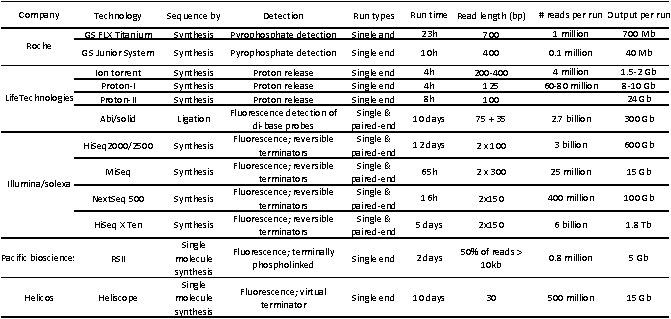
\includegraphics[width=\columnwidth]{NGStable.pdf}
    \label{fig:ngssummary}
    \end{sidewaystable}
    
    A big progress has went off ever since the days in which 454 pyrosequencer was the only reliable \gls{ngs} technology, and several technologies exist and continue to emerge in an effort to present the cheapest, quickest, and most reliable technology of \gls{ngs}. Now that the technology to produce the datasets is available, the big challenge is, and will continue to be in the next years, to store all that data and devise computational solutions for the organization and analysis of such data \citep{Illumina2015, Buermans2014, Bahassi2014, VanDijk2014}.
    	
	\subsection{Paired-end vs single-end}
    
    With the present higher sequencing capacity, it has become usual to sequence in a paired way, in which the same \gls{dna} fragment is sequenced from both ends. This translates in two files with the same number of reads, where the first sequence of the forward file corresponds to the same \gls{dna} from which comes the first sequence of the reverse file. All steps in the preprocessing phase must output two files with the same number of reads, or one with the reads from both files interleaved. These sequences may overlap or not, but represent additional clues to the original sequence. By handling paired end data the right way, this is, treating both files as fragments of the same sequences, removal of undesired sequences will be more accurate, and so will the assembling.
    
    \section{Metagenomics}
    
    Less than 2\% of bacteria can be cultured in laboratory, which immediately raises the question of how can we study the remaining 98\% that make up the backbone of most of Earth's ecosystems \citep{IlluminaProprietary}. An answer has come in the form of \gls{mg}, which involves the partial or complete sequencing of several genomes present in a \gls{dna} sample - either from viruses, bacteria or human beings \citep{IlluminaProprietary, Oulas2015, Tringe2005, Thomas2012}.
    
    \gls{mg} comes in two ways, shotgun \gls{mg} and marker gene \gls{mg}. Shotgun \gls{mg} is the complete sequencing of all the genomic material in a sample, including protein coding genes, operons and other information present in the genome, with the sub-goal of identifying what organisms compose the community of a certain sample, but having as its main objective identifying the "community potential" of the sample, the collection of genes present and that may be expressed under certain conditions. 
    
    In a \gls{mg} workflow, after sequencing, shorter reads are assembled into larger contigs by reference-based or by \textit{de novo} assembly. One strategy or even both may be used, depending on the dataset in question, the existence of a reference library and the specifications of the research project. Genes will be then annotated and the possible transcripts and proteins expressed will be identified. 
    
    Another approach is Marker Gene \gls{mg}, where in the taxonomic prokaryotic studies, 16S \gls{rrna} is usually the target gene when the aim is to get phylogenetic information, since this gene is common to all prokaryotes. Both approaches present a set of complex challenges, which have been tackled over the years with more advanced and specific informatics solutions \citep{Oulas2015, Overview2012}. Among them, are: 
    
    \begin{enumerate}
        \item \gls{pcr} noise and errors - single base pair errors, replicate sequence artifacts, \gls{pcr} chimeras.
        \item Deep sequencing - some genes are not abundant, and may not show up on sequencing results, thus underestimating the diversity of the sample.
        \item Mosaicism - horizontal transfer may result in incorrect identification of a genome.
        \item Intragenomic Heterogeneity - more specific to 16S \gls{rrna} gene studies, since bacteria may have several copies of these genes with significant variations for the same genome.
    \end{enumerate}
    
    Having opened the possibility of studying new ecosystems, \gls{mg} allows their study in native conditions, without the need of culturing in the laboratory. The study of many important ecosystems, like the soil and the human microbiome, benefited greatly from this approach, that has already expanded the knowledge concerning the different composition of microbial life in every corner of the biosphere. 
    
    \gls{mg} shotgun studies have already been applied to human feces \citep{Breitbart2003, vzifvcakova2016microbial}, mines \citep{Tyson2004}, Sargasso Sea \citep{Venter2004}, oil sands tailings ponds \citep{Tan2015}, hydrocarbon-contaminated aquifers \citep{Tan2015}, marine sediments \citep{Urich2014}, soil \citep{vzifvcakova2016microbial}, sewage \citep{vzifvcakova2016microbial}, sewage, swine wastewater sample, treated wastewater, river water and drinking water \citep{vzifvcakova2016microbial}, among others.
    
    On the other hand, \gls{rrna} 16S marker gene \gls{mg} has, for example, been applied to soil \citep{Pearce2012}, \citep{Goebiewski2014}, \citep{Damon2012}, geothermal steamvents \citep{Benson2011}, extremely acidic waters \citep{Garcia-Moyano2012}, oxygen minimum zone of the eastern tropical South Pacific \citep{Stevens2008} and Tibetan Plateau \citep{Xiong2012} populations, and is now a routine approach in most laboratories studying microbial communities. But, identifying the microbial taxonomy and genomic potential in a sample might not be enough, the next step forward would be to understand what those identified species are doing there, and this can be achieved by using shotgun \gls{mg} \citep{Tringe2005,Thomas2012}.
    
    \subsection{Metagenomics pipelines}
    
    Initially, tools developed for single genome approaches were applied in \gls{mg}, but they were not suitable for dealing with \gls{mg} data since genomic information is retrieved from several different organisms \citep{Oulas2015}. Today is a different reality, there are already several pipelines developed for the study of \gls{mg}, many of them available online.
    
    The pipelines are considerably diverse (see Table \ref{fig:mgpipelines}): some have fully integrated workflows for \gls{mg}, including quality assessment of sequencing raw data, the assembly and the annotation of genes \citep{arumugam2010smashcommunity, treangen2013metamos}. The difficulty in the installation and in the utilization differs depending on the chosen pipeline, and therefore some will require more computational knowledge from the user than others. 
    
    Some pipelines were designed to perform shotgun \gls{mg} analysis only, others are exclusive to 16S \gls{rrna} gene analysis (QIIME, Mothur \citep{Plummer2015}), while others possess the flexibility to work with both types of analyses (MG-RAST \citep{Wilke2016}, EBI metagenomics \citep{Hunter2014}). As in other areas of informatics, a trade-off is made with these pipelines: more powerful computational solutions with more tasks integrated demand more technical knowledge from the user, while more focused tools have a smoother learning curve with intuitive user interfaces, many even available in the web \citep{Ladoukakis2014, Oulas2015}. 
    
    \begin{table}[h]
    \caption{Main steps of \gls{mg} data analysis integrated in common pipelines. From \citep{Ladoukakis2014}.}
    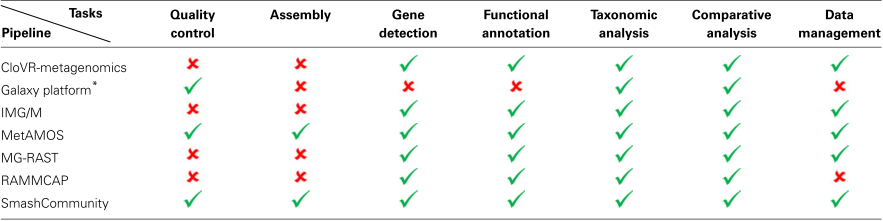
\includegraphics[width=\columnwidth]{MGs_pipelines_comparison.png}
    \label{fig:mgpipelines}
    \end{table}
    
    \cite{Ladoukakis2014} compared seven shotgun \gls{mg} pipelines - CloVR-metagenomics, Galaxy platform (metagenomics), IMG/M, MetAMOS, MG-RAST, RAMMCAP and SmashCommunity (Table \ref{fig:mgpipelines}). From those, MetAmos and SmashCommunity  were considered the most robust and versatile solutions, because they integrate all steps of \gls{mg} bioinformatics analysis and showed the best quality of the results, although they are not the easiest to operate by less experienced users. 
    
    \begin{figure}[h]
    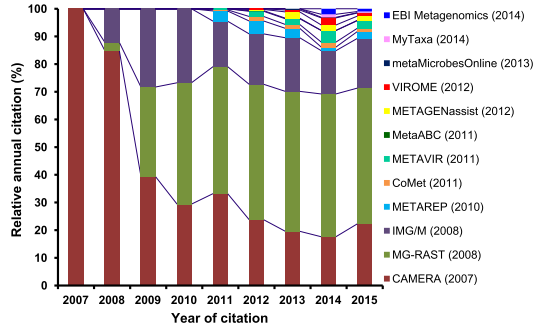
\includegraphics[width=\columnwidth]{webMGpipelines.png}
    \caption{Utilization of web resources of \textit{MG} analysis throughout the years. From \cite{Dudhagara2015}.}
    \label{fig:webmgpipelines}
    \end{figure}
    
    \cite{Dudhagara2015} also reviewed 12 \gls{mg} pipelines available accessible through the web - MG-RAST, IMG/M, METAREP, CoMet, METAGENassist, MetaABC, MyTaxa, metaMicrobesOnline, \gls{cds} Metagenomics, CAMERA, METAVIR and VIROME. These studies consider MG-RAST and IMG/M the best options for the functional analysis for already assembled data, mostly because they presented an easy interface, a database setup designed for dissemination of results to the scientific community and also because of their considerably bigger databases and a wide range of annotation tools.
    
    Concerning 16S \gls{rrna} studies, QIIME is the most used pipeline for the corresponding taxonomic interpretation \citep{Oulas2015}, being the fastest and producing similar results to mothur and MG-RAST \citep{Plummer2015}.
    
    \section{Metatranscriptomics}
    
    To know what pathways the microorganisms are utilizing can be translated in knowing what genes are being expressed more intensively, which leads to the study of \gls{mrna}.
    When collectively studying the transcriptome of several organisms in the same ecossystem, it is called \gls{mt}. 
    
    \gls{mt} analysis integrated with \gls{mg} have recently been developed, since the differential analysis of the abundance of the \gls{mrna} sequences reveals important pathways used by the community and indicate for instance which organisms are vital for maintaining the balance of microbiomes, or through what mechanisms do microorganisms survive extreme conditions. 
    
    Indicating the real activity of a microbial population, \gls{mt} functions as a complement to \gls{mg}, which only informs about what pathways can be used - the genomic potential of the population \citep{Bikel2015, Aguiar-pulido2016}. \gls{mt} presents simpler datasets than \gls{mg}, since \gls{mrna} confines to the coding regions of the genome and not all genes are transcribed under a certain condition, thus allowing for less complex datasets that generate more focused and useful functional information.
    
    \gls{mt} distinguishes itself from \gls{mg} in some steps of its analysis: 
    \begin{itemize}
        \item For studies aiming at the study of \gls{mrna}, a depletion of \gls{rrna} is necessary, at the wet- and dry-lab level \citep{Narayanasamy2016}.
        \item \gls{mrna} is very unstable, which might be a factor for ruining the sample before sequencing
        \item It is harder to distinguish between bacterial and other living beings \gls{rna}, which might be a serious problem in human microbiome studies.
        \item Overrepresented sequences that would be discarded in \gls{mg} as undesired are normal in a \gls{mt} dataset, and therefore to be kept.
        \item The size of \gls{rna} fragments is usually smaller than that of \gls{dna}, so each \gls{rna} sequence is usually sequenced much more times than \gls{dna} sequences, thus allowing for more reliable results of sequencing.
    \end{itemize}
    
    With the development of kits of enrichment of bacterial \gls{rna} and several techniques of \gls{rrna} depletion, several and diverse studies of \gls{mt} have already been developed \citep{Aguiar-pulido2016}. Several works have been developed in \gls{mt} functional and differential analysis, such as the ones applied to soil \citep{Carvalhais2012}, stimulus-induced biofilms \citep{Ishii2015}, mouse intestine \citep{10.1371/journal.pone.0036009}, kimchi \citep{Jung2013}, bovine rumen \citep{Poulsen2013} and deep-sea populations \citep{Baker2013}, among others.
    
    \subsection{Metatranscriptomics pipelines}
    
    \gls{mt} pipelines follow basically the same steps and have to deal with most of the problems of their \gls{mg} counterparts, in addition to the overwhelming presence of \gls{rrna} in comparison to \gls{mrna}. In four steps - preprocessing of reads, annotation of contigs, aggregation of the annotated contigs, and analysis of results - \gls{mt} pipelines obtain information about the entire transcriptome, and therefore on the metabolic pathways expressed and also on taxonomic composition of complex microbial communities \citep{Westreich2016}. 
    
    Until recently, there was no pipeline fully integrating the steps of assembly and annotation for \gls{mt} data. A comparison of four assemblers - Trinity, Oases, Metavelvet and IDBA-MT - revealed Trinity as the most reliable in assembling more reads to contigs with annotation value \citep{Celaj2014}. 
    In 2016, the first pipelines to integrate all the steps of metatranscriptomics were released: MetaTrans and SAMSA. MetaTrans performs both taxonomic - making use of 16S \gls{rrna} - and gene expression analysis of \gls{rna}-Seq, after quality-control assessment and \gls{rrna} removal. It uses \gls{cdna} libraries for \gls{pe} sequencing, and maps them against functional databases \citep{Martinez2016}. SAMSA identifies the more prominent species and the functional differences between \gls{mt} datasets, which allows for multisample comparison. It does require reads to be longer than 100 \gls{bp} or paired-end, however, which is not always easy to fulfill \citep{Westreich2016}.
    
    \section{Integrated analysis of metatranscriptomics coupled to metagenomics}
    
    To be able to figure out which pathways are being most expressed in a given sample, it is necessary to integrate \gls{mg} and \gls{mt} data analysis \citep{Dudhagara2015, Nayfact2016}. However, there are only a few publicly available pipelines developed for multiomics approaches. Very recently, the first publicly available pipelines integrating \gls{mg} and \gls{mt} analysis have been presented, and the two available to date will be described in detail below.
    
    \gls{imp} and \gls{fmap} are two available pipelines developed to analyze simultaneously MG and MT data for a better interpretation of MT studies. \gls{imp} is an open-source pipeline designed for the preprocessing, assembly and analysis of \gls{mg} and \gls{mt} data \citep{Narayanasamy2016}. The two main features that distinguish it from other pipelines are its iterative co-assembly of \gls{mg} and \gls{mt} reads and its containerization in docker - allowing for reproducibility of its results. Docker \citep{chamberlain2014using} is a virtual machine whose environment may be built to reproduce the computational environment of the researcher at the time of his work, in an easy to build, accessible way. 
    \gls{imp} is the only pipeline to integrate \gls{mg} and \gls{mt} reads by iterative co-assembly, which greatly increased the identification of protein coding genes when compared to results obtained based on assembly of \gls{mg} reads only. However, \glsfirst{de}, the analysis of diferential expression of genes,  was not considered in this pipeline.
    
    The preprocessing steps include trimming and quality filtering (by \textit{Trimmomatic}) and \gls{rrna} filtering (by \textit{SortMeRNA 2.0}). Assembly is achieved through read mapping (by \textit{bwa}), extracting unmapped reads (by \textit{samtools} and \textit{BEDtools}) and filtering host sequences.
    After assembly, \textit{VizBin} is used for binning, and in the analysis step, \textit{Prokka} is used for the annotation and \textit{VizBin} for a detailed and interactive look at the results. Written in Bash, Make and Python, docker and python are the only requirements previous to the installation of the \gls{imp} for using the tool, allowing for a easier installation and use of the pipeline \citep{Narayanasamy2016}.
    
    \gls{fmap} is the only implementation to date that handles both \gls{mg} and \gls{mt} analysis while also performing \gls{de} analysis with support from the \gls{mg} information, which is vital to understand the functional behaviour of a community. Besides that, \gls{fmap} also implements more typical \gls{mg} features, like sequence alignment and determination of gene families presence.
    
    In the preprocessing step of the workflow, the usual removal of low-quality and human sequences is done through \textit{BMTagger}, and the alignment of the remaining reads goes through \textit{USEARCH} or \textit{DIAMOND}, with a \gls{kfu} reference cluster as database - enriched in bacteria, fungi and archaea sequences, for more robust and informative results. The result of this alignment may be extracted for annotation with another software.
    
    After assembly, gene abundance is determined by raw count or \gls{rpkm}, and for differential quantification, \textit{metagenomeSeq}, using raw count, and Kruskal-Wallis and quasi-Poisson, both using \gls{rpkm}, are the tools selected for that step. The three show variable quality of results depending on the situation, and so the three are implemented in \gls{fmap}. 
    
    Enriched operons analysis is based on the differential gene abundance, considering differential abundant the operon corresponding to the gene differentially abundant. The definition of operon in \gls{fmap} is tied to the \gls{ko} concept, where each \gls{ko} corresponds to a molecular-level function. In \gls{fmap}, the differential abundance of operons also means the differential abundance of its corresponding pathway, and another output of \gls{fmap} is an input to \gls{kegg} online pathway map tool, where it is possible to easily visualize which pathways are more represented in the sample, among all pathways available in \gls{kegg} \citep{Kim2016}.
    
    A limitation of \gls{fmap} is that it was not designed for comparison of data between different samples, although having ShotgunFunctionalizeR in its workflow, an R package specific for functional comparison of metagenomes of different samples \citep{kristiansson2009shotgunfunctionalizer}.
    
    A typical workflow for \gls{mg}/\gls{mt} studies, including the main steps and tools for a complete bioinformatics data analysis, is presented in figure \ref{fig:pipelinedesign}.
    
    \begin{figure}[ph!]
    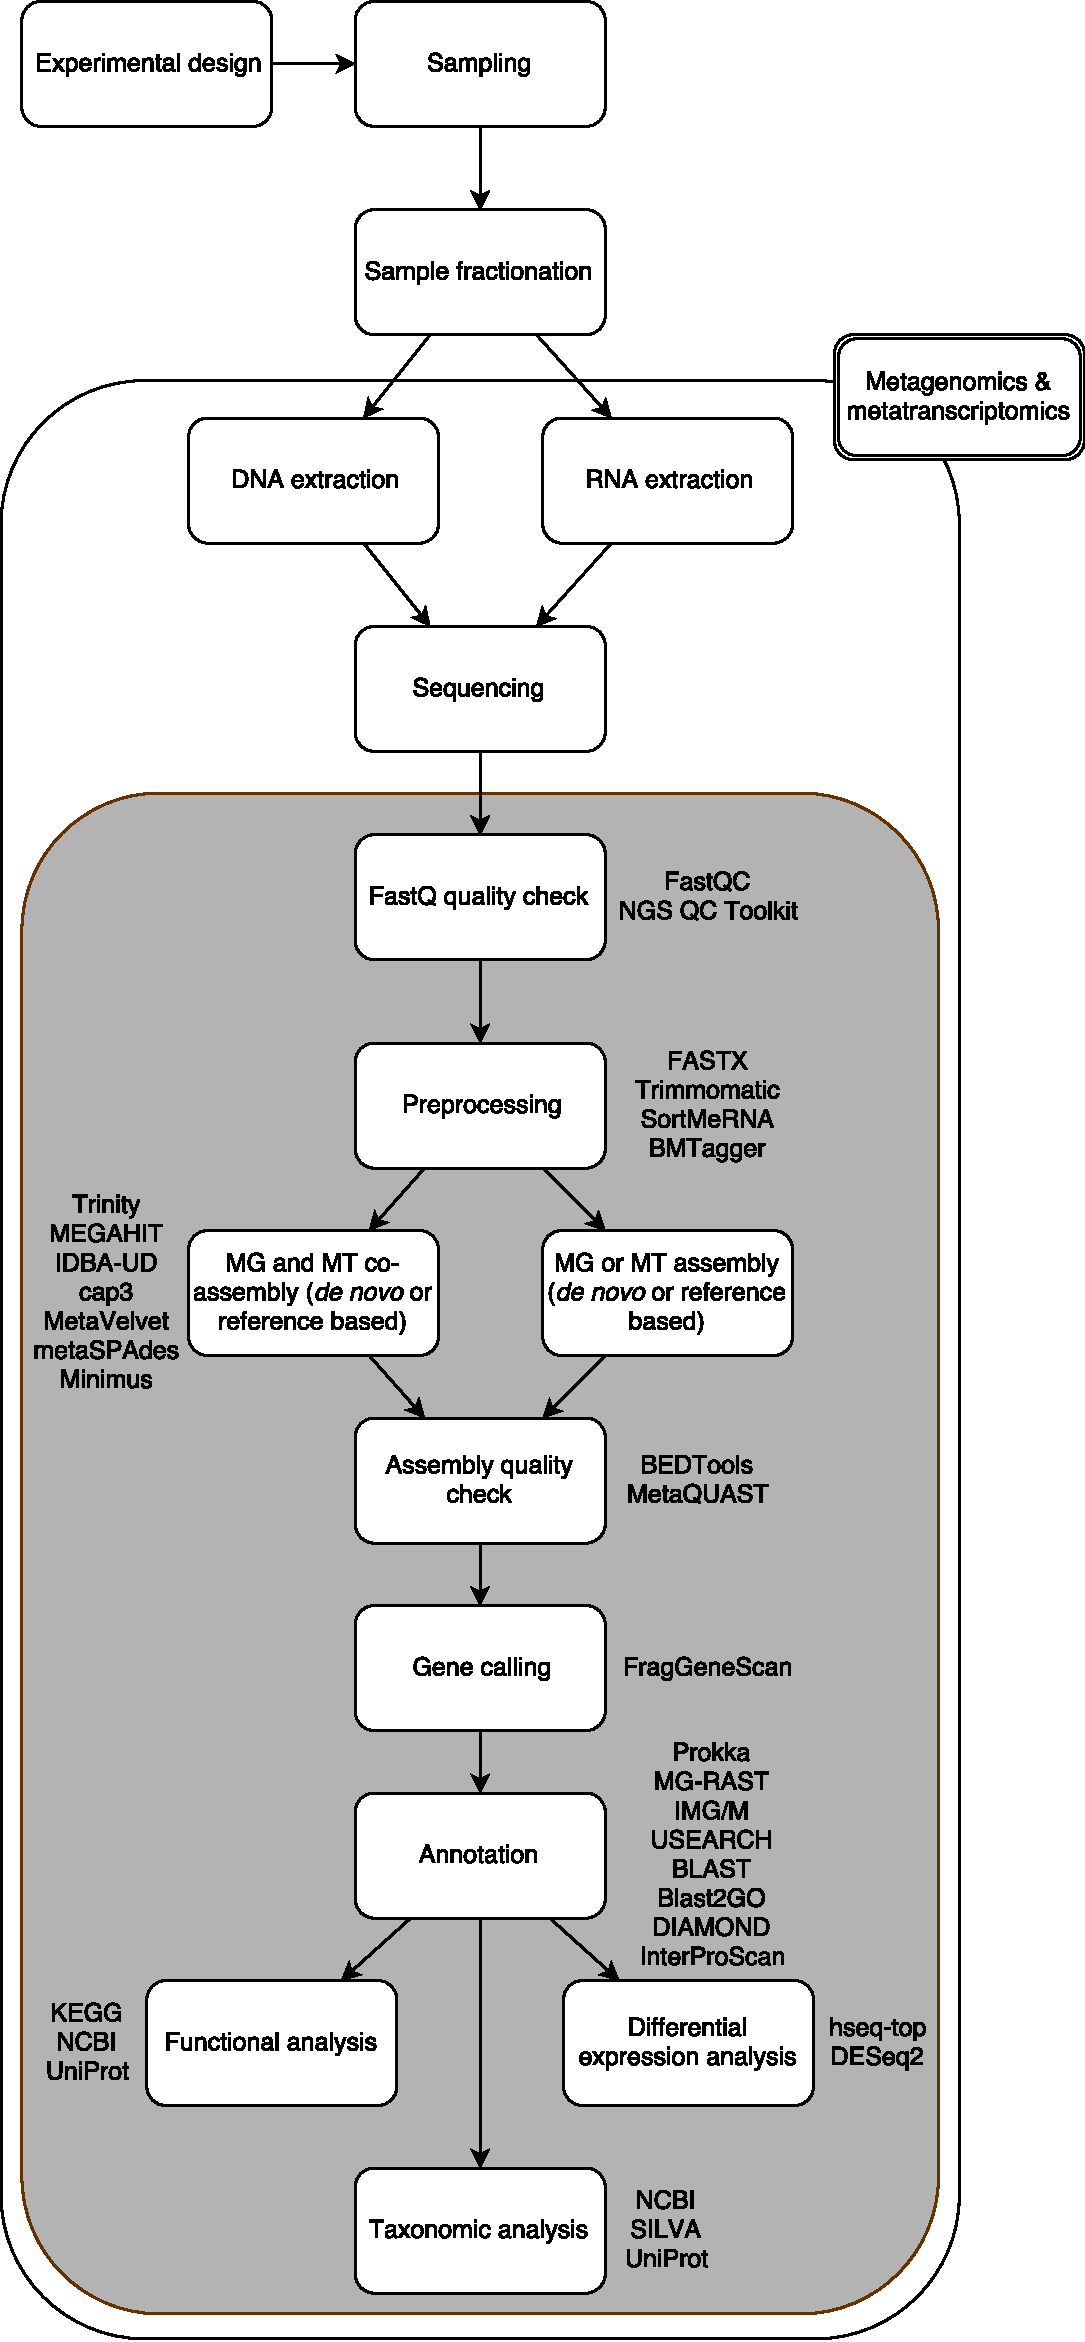
\includegraphics[width=\columnwidth, height=\textheight]{FiguresUndTables/Development/entire_pipeline.pdf}
    \caption{Typical Meta-Omics pipeline workflow, from the laboratory to the bioinformatics processing steps. Inside the squares are the major steps. The tools and software possibilities are represented next to each step of the workflow.}
    \label{fig:pipelinedesign}
    \end{figure}
    
    \section{Steps and tools for MG/MT data analysis}
    
    \gls{ngs} methods can produce large amounts of data, which are necessary in meta-omics studies. There are optimized informatics tools that handle such large amounts of data and that were designed for the different steps of meta-omics data analysis, namely quality control, preprocessing, assembly, bining, annotation and statistical and visual analysis. Several of these tools have been integrated in pipelines, to allow for easier workflows (Table \ref{fig:pipelinesreview}). A brief overview of the main steps and most common tools utilized in each step of \gls{mg} and/or \gls{mt} data analysis will be given.
    
    \subsection{Steps and tools for Preprocessing}
    
    The preprocessing mainly consists on the removal of undesired sequences from \gls{ngs} datasets. All pipelines include a preprocessing phase, but some integrate only a small number of steps, like MetAMOS, while others offer more complex preprocessings, like \gls{imp} and MetaTrans (Table  \ref{fig:pipelinesreview}).
    
    \begin{table}[!h]    
    \caption{Comparison of different steps and tools present in some \gls{mg} and \gls{mt} pipelines.}
    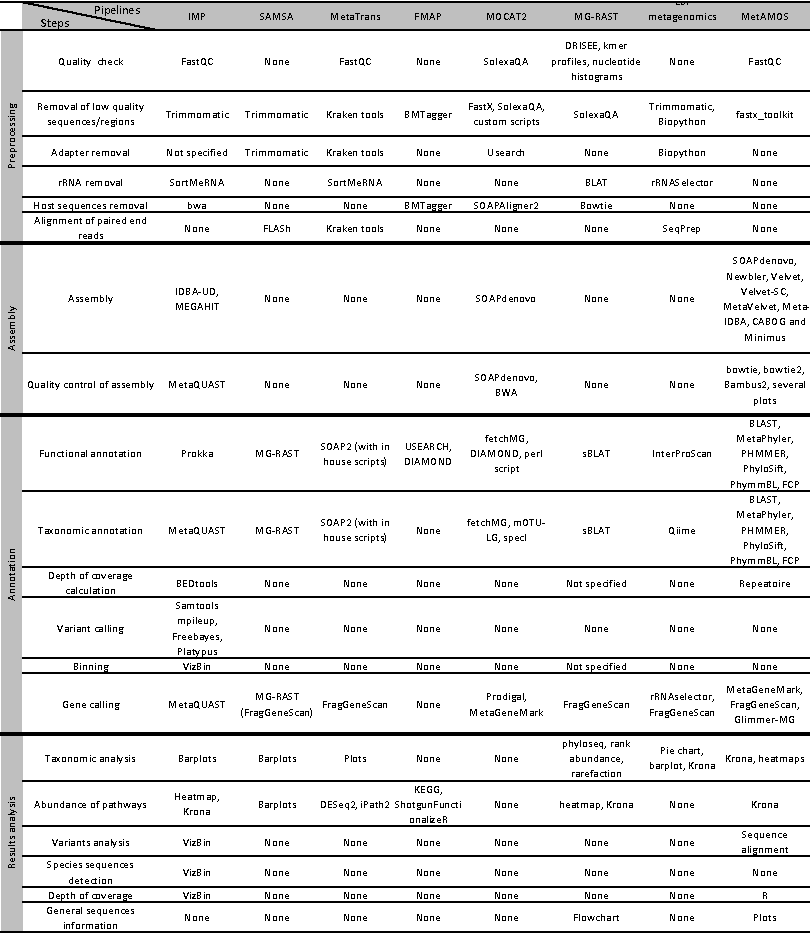
\includegraphics[width=\columnwidth]{FiguresUndTables/State_of_art/pipelines_review.pdf}
    \label{fig:pipelinesreview}
    \end{table}
    
    After the quality of the sequencing reads has been inspected, preprocessing prepares the dataset for the further steps, by removing undesirable sequences. Trimming is to remove the sequences of less interest from the datasets, either because they are too short, they are from species not in the scope of the study or there is too much doubt about the consensus sequence, the latter being quantified by the scores relative to each position of the read. Trimmomatic \citep{bolger2014trimmomatic} is one of the solutions for removing low quality and short sequences and BMTagger \citep{rotmistrovsky2011bmtagger} is capable of identifying and removing human sequences. When the work involves study of \gls{mrna}, a depletion of \gls{rrna} sequences is necessary. SortMeRNA \citep{doi:10.1093/bioinformatics/bts611} identifies the \gls{rrna} sequences and removes them from the dataset.

    \paragraph{Quality check of FastQ reads}
    
    In the first \textit{in silico} step of a post-\gls{ngs} bioinformatics workflow, the datasets of reads produced by sequencing usually undergo quality check. FASTQ format is an usual output file format of \gls{ngs}, but a quality control tool should also have the capacity to analyze SAM, a compressed version of FASTQ, and BAM files, the binary version of SAM \citep{jones2012compression}. In addition, two scoring formats, PHRED-33 and PHRED-64, originate two different FASTQ versions depending on the \gls{ngs} technology used \citep{cock2010sanger}. Finally, a quality check should output statistical and graphical analyses of several subjects about the quality of the datasets being studied. FastQC \citep{andrews2010fastqc} and NGS QC Toolkit \citep{10.1371/journal.pone.0030619} are two solutions for this task, with FastQC being the most used and validated.
    
    FastQC \citep{andrews2010fastqc} is currently the most popular tool at checking the quality of \gls{ngs} data, but other options exist, like DRISEE for calculating sequencing errors and custom application of histograms for measuring presence of bases in every position of the dataset, and SolexaQA \citep{cox2010solexaqa}, which posses several informative graphical results aswell. FastQC retrieves a quality report showing the important characteristics of \gls{ngs} data in boxplots, line plots and including a colored code indicating if there is any quality problem and at which level. This analysis is fast, easy to use and to interpret, which has led FastQC to become the most used quality control tool. The strength of FastQC is reflected in the fact that several pipelines used FastQC to generate the initial quality control report, and in further steps during the preprocessing stage. 
    
    \paragraph{Undesired sequences removal}
    
    After the quality of the sequencing reads has been inspected, preprocessing prepares the dataset for the further steps, by removing undesirable sequences. Trimming is to remove the sequences of less interest from the datasets, either because they are too short, from species not in the scope of the study, there is not enough confidence about the consensus sequence, quantified by the scores relative to each position of the read, or there are artificial sequences from the experimental work of obtaining the nucleotidic sequences.
    
    Trimmomatic \citep{bolger2014trimmomatic} is becoming more and more popular as a toolbox for tailoring \gls{ngs} datasets in many different ways, most concerned with data quality, making use of the quality related information contained in FastQ files. Different tools allow for a versatile response to data problems, which is translated into a powerful and versatile solution for quality and artificial sequences trimming. These are some of the reasons that explain its incorporation in many pipelines, mainly for removing artificial sequences and for cropping or removing entire sequences. SolexaQA and FastX \citep{gordon2010fastx} are examples of alternative toolboxes available for the bioinformatics community, and can be found integrated in some pipelines as well.
    
    \paragraph{rRNA and host sequences removal}
    
    Because most of the pipelines are focused on \gls{mg} data analysis, which contains much less \gls{rrna} sequences than \gls{mt} data, removal of \gls{rrna} sequences is not widespread throughout their preprocessing workflows. For the identification and removal of \gls{rrna} sequences in \gls{ngs} datasets, the choice of both software and reference database is highly important. SILVA databases \citep{quast2012silva} have become the golden standard among \gls{rrna} databases, containing all types of \gls{rrna} sequences in a single resource: all domains - prokaryotic, archaea and eukaryotic - and all \gls{rrna} subunits - 16S, 23S, 18S and 28S. Different tools can be used to map the datasets to databases, which use different approaches. For example, prior to alignment of sequence reads to databases, SortMeRNA \citep{doi:10.1093/bioinformatics/bts611} and BLAT \citep{kent2002blat} generate an index for each database, while rRNASelector \citep{lee2011rrnaselector} uses HMMER and \gls{hmm}.
    
    Host sequences removal is a very important step, since even when not working with samples from human gut, it still must be assured that the samples are voided of human sequences for submission in certain web servers for annotation and posterior analysis. Like \gls{rrna} depletion, it is, however, not implemented in many of the state-of-the-art pipelines for \gls{mg} and \gls{mt} data analysis. The most important question is, again, what database to use. Examples of tools for removing human and other hosts derived sequences are BMTagger \citep{rotmistrovsky2011bmtagger}, SOAPaligner \citep{gu2013using} and Bowtie \citep{langmead2012fast}.

    \subsection{Bioinformatic tools for Assembly}
    
    Aligning the reads into contigs that represent as closely as possible the sequences present in the original sample is a task already approached with different strategies to make use of the most resources possible. If there are available examples of the target organisms genomes or of closely related species, then a database reference based assembly may be the best solution, which is the strategy of Minimus \citep{sommer2007minimus}, from the MetAMOS pipeline \citep{treangen2013metamos}. If there is no closely related genomes available, \textit{de novo} assembly is a solution, for which there is Trinity \citep{Celaj2014} for \gls{mt} data assembling, and MetaVelvet \citep{namiki2012metavelvet}, metaSPAdes \citep{nurk2016metaspades}, MEGAHIT \citep{li2015megahit} and IDBA-UD \citep{peng2012idba} for \gls{mg}. cap3 \citep{huang1999cap3} can also be used as a standalone assembler or as a complement to other programs by further merging contigs into bigger ones.
    
    After an assembly, it is important to evaluate the results concerning genes and species detection. BEDTools \citep{quinlan2010bedtools} possesses a suite of tools for that task, while MetaQUAST \citep{mikheenko2016metaquast} could be used as alternative, by presenting several classic metrics such total assembly size and N50. By reconstructing the assembly back to the original contigs it is possible to have an ideia of the ammount of reads used in the assembly, allowing to better understand how much of the original information is present in the contigs. Such is achieved by aligning the reads to the contigs, using Bowtie2 \citep{langmead2012fast} or BWA \citep{doi:10.1093/bioinformatics/btp324}, for example.
    
    Despite its proven usefulness, assembling is not included in most pipelines (Table \ref{fig:pipelinesreview}). \gls{imp}, MOCAT2 and MetAMOS present examples of implementation of an assembling routine, with MetAMOS possessing by far the largest collection of assembling options, with eight different tools to choose from, and three types of assembly, single genome/isolate, metagenomic and single cell assembly. Some of its assemblers are not capable of performing all types of assembly, however, and the tool has been specifically designed towards metagenomic analysis (it was built from AMOS, a genome assembly framework). 

    \gls{imp} incorporates two assemblers and the option to co-assemble \gls{mg} with \gls{mt} data, in an iterative procedure - after a first assembly, the first contigs and the remaining unused reads serve as input for a second assembly. Additional rounds of assembly could be implemented, but do not show a significant increase in number of contigs after the second assembly.
    
    MOCAT2 \citep{Kultima2012} assembles the reads into contigs and scaftigs (scaftigs are contigs extended using paired-end information).
    
    \paragraph{Quality control of assembly}
    
    MetAMOS also implements by far the most complex evaluation and correction of assembling, which starts by mapping the original reads used for the assembling back to the contigs determined by the assemblers (using Bowtie and Bowtie2), and using such mapping to estimate depth of coverage, filter contigs with no reads mapped to them, create links between contigs for scaffolding and re-estimate fragment lengths. Still in MetAMOS, Repeatoire annotates repetitive contigs, allowing for identifying under-collapsed sequence output from the assembling step. Some later applications of other tools also facilitate some annotation steps, and are discussed in the annotation section bellow.
    
    \gls{imp} makes use of MetaQUAST to calculate several metrics concerning the contigs produced, such as N50 and number of contigs. Even though this are classic metrics used in the evaluation of assemblies, it lacks an approach such as that of bowtie to deconstruct the assemblies and relate the original reads with the contigs. MOCAT2 makes use of SOAPdenovo and BWA to correct for indels and chimeric regions.
    
    MOCAT2 \citep{Kultima2012} uses BWA to correct base errors and short indels in the assembly, by aligning the reads to the generated scaftigs, and SOAPaligner2 to resolve chimeric regions, by aligning the several contigs.
   
    \subsection{Bioinformatic tools for Annotation}
    
    After obtaining a list of partial and entire genomes predicted to be present in the sample of study, it is a common step to identify what genes are present, first by identifying \gls{orf}s in the sequences, which can be done with FragGeneScan \citep{rho2010fraggenescan} and then by submitting each \gls{orf} detected to a search software that searches the databases for the closest entries to the sequence, either by homology or pre-determined features. Tools developed for this task are Prokka \citep{seemann2014prokka}, IMG/M \citep{markowitz2008img}, BLAST \citep{altschul1990basic}, DIAMOND \citep{buchfink2015fast}, USEARCH \citep{edgar2010search}, and Blast2GO \citep{conesa2005blast2go}, the latter through use of Gene Ontology. MG-RAST \citep{glass2010using} is also widely used for this purpose, while integrating additional features such as phylogenetic and functional classifications of metagenomes \citep{meyer2008metagenomics}, and InterProScan \citep{Jones2014}, the tool that allows for access to InterPro domain information.
    
    All pipelines infer the origin and function of the original reads or of the contigs produced by the assembly steps, in their annotation phase (Table \ref{fig:pipelinesreview}). Such determination usually starts by identifying the \gls{orf}s, in a process known as gene calling. After that, functional and taxonomic annotation is generally performed by aligning the obtained sequences to protein databases. Binning help in separating the total transcriptome into smaller, taxon specific clusters, necessary for understanding the individual importance of such taxon. Variant calling allows to identify small differences in similar sequences, although it may sacrifice some speed of the pipeline because of the sheer size of data usually processed.
    
    \paragraph{Gene calling}
    
    The identification of \gls{orf}s approach is very dependent on the specific characteristics of the analyzed contigs. One of the most used tools is FragGeneScan (Table \ref{fig:pipelinesreview}), which incorporates a machine learning algorithm, and even though it works well when challenged with short reads, it is versatile enough to be used with longer reads from both \gls{mg} and genomic datasets, and by combining models of sequencing error and codon usages in its \gls{hmm}, it performs very well with error prone reads. Other tools, such as MetaGeneMark and Glimmer-MG, have also been specifically developed for handling gene calling in \gls{mg} samples. rRNAselector identifies regions encoding for \gls{rrna} in \gls{mg} and \gls{mt} datasets.
    
    \paragraph{Functional and taxonomic annotation}
    
    Functional and taxonomic annotation is usually tackled by aligning the contigs against databases containing the specific sequences expected to be found on the datasets. In meta-omics studies, however, such databases must be more general, for it is usually not known the totality of species present in the environments from where the samples came. More functional databases, such as UniProt and KEGG, are used to identify the functions of the proteins found in the datasets, which allows for mapping such functions to metabolic pathways, and discover which are the most important ones. Taxonomy may be determined from the alignments in the functional annotation, or it may be determined by aligning the 16S \gls{rrna} or \gls{dna} sequences to 16S databases, such as SILVA, Greengenes and \gls{ncbi}.
    
    BLAST has been the classic tool used for such alignments, but DIAMOND applies an algorithm tailored for short reads, much faster in such situations when compared with the other solutions. USEARCH and VSEARCH are alternatives similar to DIAMOND, faster than BLAST and tailored for \gls{mg}. Specifically for taxonomic annotation, MetaQUAST incorporates an algorithm for searching the SILVA database automatically, when assessing the quality metrics of the contigs (Table \ref{fig:pipelinesreview}).
    
    \paragraph{Depth of coverage}
    
    Depth of coverage is measured by how many times a certain sequence appears in the dataset. Average depth of coverage is that concept applied to the full dataset. A higher coverage confirms the veracity of the sequences (less randomness from sequencing and assembling errors), and allows to detect \gls{snp}s when present on those sequences. \gls{mg} data usually exhibits less coverage, however, which might compromise organisms identification. Coverage is also used to measure gene expression when applied to \gls{mt} datasets, since original higher abundance of material related to a certain gene is usually the reason for a higher coverage, which in such cases might be magnitudes of times more variable than in \gls{mg} datasets. BEDtools and Repeatoire are two options for calculating depth of coverage, but it is not a much implemented step in the compared pipelines (Table \ref{fig:pipelinesreview}).
    
    \paragraph{Variant calling}
    
    Currently, \gls{imp} is the only pipeline to integrate the process of identifying and putting in relevance small variations between very similar contigs, since because of the sheer scale of the data, identifying such strain specific characteristics is not a priority. Nevertheless, it has its place when studying multiple strains of the same organism. In \gls{imp}, samtools\'s mpileup tool is used to provide a summary of the depth of coverage for each base pair on the sequences aligned to the assembled contigs, Freebays detects such variations but on the original reads, without aligning them back to the assembly, and Platypus performs both types of variant detection.
    
    \paragraph{Binning}
    
    For population studies, binning has proven to be a helpful step in assigning an \gls{otu} to the contigs originated in assembly, which are aggregated in clusters in this step and classified with the \gls{otu} for more comprehensive population level information. VizBin \citep{laczny2015vizbin} accomplishes this, while also producing visual representations of the results, and CheckM \citep{parks2015checkm} makes available a suite of tools for evaluating the binning quality.
    
    Binning may serve two purposes: the resulting contigs may be organized into clusters (bins) to diminish data size by only considering one or a few representative sequences from each bin in future analysis; and the contigs may be assigned to a specific taxa, where the assembly serves as the binning process itself. Ideally, there will be one contig by different genome, but in \gls{mg} it is usually hard to avoid co-assemblies and misassemblies \citep{Kunin2008}. Not just the pure sequence alignment but some nucleotide features related to processes directly involved with \gls{dna}, like its repair, and codon usage, might be used for the binning as well.
    
    The only two pipelines to integrate binning have applied it for the first function, in an effort to simplify the datasets (Table \ref{fig:pipelinesreview}). VizBin, for example, provides interactive 2D maps of points representing the contigs, where it may be possible to discern clusters that might represent several closely related contigs. This maps allow the user to isolate this clusters and reduce them to one single contig.
    
    \subsection{Bioinformatic tools for Statistical analysis}
    
    Many analyses may come from meta-omics studies, and these are even more varied when talking about multi-omics approaches: determining \gls{gc} content of the genomes, main pathways active, \gls{mt}/\gls{mg} ratios, and much more. There are many R packages, such as ShotgunFunctionalizer \citep{kristiansson2009shotgunfunctionalizer}, that tackle several of these challenges, as does Blast2GO \citep{conesa2005blast2go}.
    
    \paragraph{Visualization of the results}
    
    As seeing the analysis results in a comprehensive, intuitive way is usually easier and more useful than to read results in text, many tools already incorporate several types of graphics, many even interactive, for a more helpful approach to presenting results. As an example, VizBin \citep{laczny2015vizbin} provides several graphical solutions to perceive the binning results, and Krona tools \citep{ondov2011interactive} is an example of interactive graphic results where a user has access to several layers of the same information. Blast2GO \citep{conesa2005blast2go} makes use of colour changes for a better understanding of the annotation process and of graph representations for highlighting the most important GO, while MG-RAST \citep{glass2010using} provides pie charts representative of several different communities' profiles and heatmaps with differential multisample analysis. MEGAN \citep{huson2007megan}  is a pipeline designed for handling the latter steps in the analysis of microbiome data, integrating tools such as DIAMOND for annotation, but making available a large suite of tools for visual analysis, involving, for example, Voronoi tree maps, principal coordinates analysis and interaction with InterPro2GO \citep{camon2004gene}, eggNOG \citep{powell2012eggnog} and KEGG \citep{Kanehisa2000a}.
    
    \section{The databases for annotation}
    
    \subsection{UniProt}
    
    A consortium made of the collaboration between the \gls{embl-ebi}, the \gls{pir} and the \gls{sib}, \gls{uniprot} is composed of four approaches to the storage of protein information: the \gls{uniprot} Knowledgebase (UniProtKB), the \gls{uniprot} Archive (UniParc), the \gls{uniprot} Reference Clusters (UniRef) and the \gls{uniprot} Metagenomic and Environmental Sequences (UniMES). 
    
    UniProtKB is the main point of acess to \gls{uniprot}, and is divided in two, distinct parts - UniProtKB SwissProt, where the increment in information is more supervised, with information extracted from the literature or from computational scrutiny, and UniProtKB TrEMBL, with more automated and less reviewed information. 
    
    UniParc is a repository of past information not only concerning entries of \gls{uniprot}, but also of several other databases, in a comprehensive, aggregated way. UniRef speeds database query by merging the information contained in UniProtKB into clusters according to the percentage of identity - 50\%, 90\% and 100\% of identity lies between the clusters of UniRef50, UniRef90 and UniRef100 respectively, and UniMES contains data concerning a number of metagenomic studies not available in UniProtKB \citep{UniProt2010, Bateman2015}. The massive increase in sequencing initiatives has been followed by a massive increase in \gls{uniprot} data, and the \gls{uniprot} interface has seen many changes to facilitate the user survey through such a big database \citep{Bateman2015}.
    
    \subsection{KEGG}
    
    Starting on 1995 as a repository of information derived from the Human Genome Program, \gls{kegg} has grown to become one of the most relevant databases concerning functional information of organisms and analysis of pathways \citep{Kanehisa2000a}. Starting based on three databases, it is now divided in eighteen: \gls{kegg} PATHWAY, \gls{kegg} BRITE and \gls{kegg} MODULE are designed for systems information, for understanding life at the system level; \gls{kegg} ORTHOLOGY, \gls{kegg} GENOME and \gls{kegg} GENES organize information retrieved from \gls{ncbi}'s RefSeq and GenBank, aggregating it into \gls{ko}s, for an easier access to better organized and diverse Genomic Information, with links to other databases such as \gls{ncbi}; \gls{kegg} COMPOUND, \gls{kegg} GLYCAN, \gls{kegg} REACTION, \gls{kegg} RPAIR, \gls{kegg} RCLASS, and \gls{kegg} ENZYME compose the Chemical Information of \gls{kegg}, with information detailing each metabolite and enzyme present in the pathways of \gls{kegg}; \gls{kegg} DISEASE, \gls{kegg} DRUG, \gls{kegg} DGROUP, \gls{kegg} ENVIRON, JAPIC and DailyMed provide Health Information, concerning diseases and drugs. \gls{kegg} presents itself as database of information organized by, besides the normal formats, its pathways and orthologies that allow for a more visual and direct search \citep{Kanehisa2000a, Kanehisa2016}.
    
    \subsection{Conserved Domains Database}
    
    Starting as a mirror for Pfam \citep{Bateman2004}, a collection of protein families and domains, Simple Modular Architecture Research Tool (SMART) \citep{Letunic2004}, a tool for annotation of protein domains, and Clusters of Orthologous Groups (COG) \citep{Tatusov2003}, a database for clustering of genes for generation of taxonomic information, the \gls{cdd} has grown to become an important repository of protein domain information, with an ever increasing amount of information concerning domain models and description. With resources such as superfamily clustering and domain annotation with attention to common domain architectures, \gls{cdd} has gone beyond a simple aggregation of databases to become a tool in itself for the analysis of sequences in respect to their structure.
    
    \subsection{InterPro}
    
    InterPro is an \gls{ebi} database that collects protein domains information from several databases: HAMAP \citep{Lima2009}, PANTHER \citep{Thomas2003}, PfamA \citep{Finn2014}, PIRSF \citep{Wu2004}, ProDom \citep{Corpet1998}, PRINTS \citep{Attwood2002}, Prosite-Profiles \citep{Sigrist2002}, SMART \citep{Schultz2000}, TIGRFAM \citep{Haft2003} and Prosite-Patterns \citep{Sigrist2002} for information about protein families, domains, functional sites and repeats regions, Gene3d \citep{Buchan2002} and SUPERFAMILY \citep{Gough2002} for structural information and Coils \citep{Lupas1991}, Phobius \citep{Kall2004}, SignalP \citep{Emanuelsson2007} and TMHMM \citep{Krogh2001} for additional features information \citep{Hunter2009, Finn2016}. 
    
    Recently, InterPro added to its consortium the databases SFLD \citep{Akiva2014}, structure/function relational information, and \gls{cdd} \citep{Marchler-Bauer2015}, which is, like InterPro, supported by a consortium of databases, but from which only the \gls{cdd} entries are extracted (since the other databases are already integrated in InterPro) \citep{Finn2016}. This diverse consortium of database partners results in varied data, that along the years has been made more uniform by InterPro, in an effort to facilitate access and reference. InterPro also has taken a direction towards studying how the signatures from this databases are connected, thus generating new, more in-depth, information \citep{Hunter2009}.
    
    InterProScan is the service provided by \gls{ebi} that extends the funcionality of InterPro by facilitating study of proteic and nucleic sequences against InterPro data \citep{Zdobnov2001, Quevillon2005}. Besides an interactive interface, it allows programmatic access through REST and SOAP protocols in several programmatic languages \citep{Jones2014}. Through InterProScan, it is possible to access most information kept in InterPro from all its member databases, which is returned in several formats, namely HTML, which contains the graphic interpretation of the results, organized by repeated matches (because some databases will match for the same domain, with the same InterPro identifier), GFF, which contains information regarding the location of the domain, the database of origin, the GO terms associated to that particular domain, the E-value associated with the match, among other information, and XML, which contains all the information contained in the GFF file, with more detailed information, like, for example, the models associated with that domain and the location of the domain concerning Hidden Markov Models and environment data. It also returns other kinds of information, like log files \citep{Quevillon2005}.
    
    \subsection{NCBI's RefSeq}
    
    RefSeq is a non-redundant database of genomic, transcriptomic and proteomic sequences built and maintained by the \gls{ncbi}. It organizes information from many sources, both from \gls{ncbi}, like \gls{cdd} and GenBank (the redundant version of RefSeq, with several entries for the same sequences), and from databases of other organizations, like the Saccharomyces Genome Database (SGD) and The Institute for Genomic Research (TIGR), collecting the information regarding each entity into a single entry. The information from RefSeq is available directly from the site itself, from other \gls{ncbi}'s resources, or from tools like \gls{blast} \citep{Pruitt2007a, OLeary2016}.

	% CHAPTER - Contribution -------------------------
	\chapter{Development}
	
	\gls{mosca} was developed by constructing wrappers to integrate bioinformatic tools for meta-omics analysis (Table \ref{versions}). Firstly by testing with variable arguments, and afterwards by developing python scripts to replicate the behavior of the tools, \gls{mosca} was developed for full automation of metagenomic and metatranscriptomic analysis of single- or paired-end data.

    \section{Pipeline architecture and implementation in MOSCA}
    
    \subsection{Preprocessing}
    
    The preprocessing of \gls{mosca} aims to remove all undesired sequences from the raw data, to obtain a dataset with only meaningful, good quality reads and free of \gls{rrna}. It uses FastQC for several quality evaluations of the data during the preprocessing workflow, to evaluate the quality of the raw data, before trimming by Trimmomatic, and after SortMeRNA. The main steps of the preprocessing, including the tools and the name of the python scripts, are represented in Figure \ref{fig:moscaclasses}.
    
    \begin{figure}[ph!]
    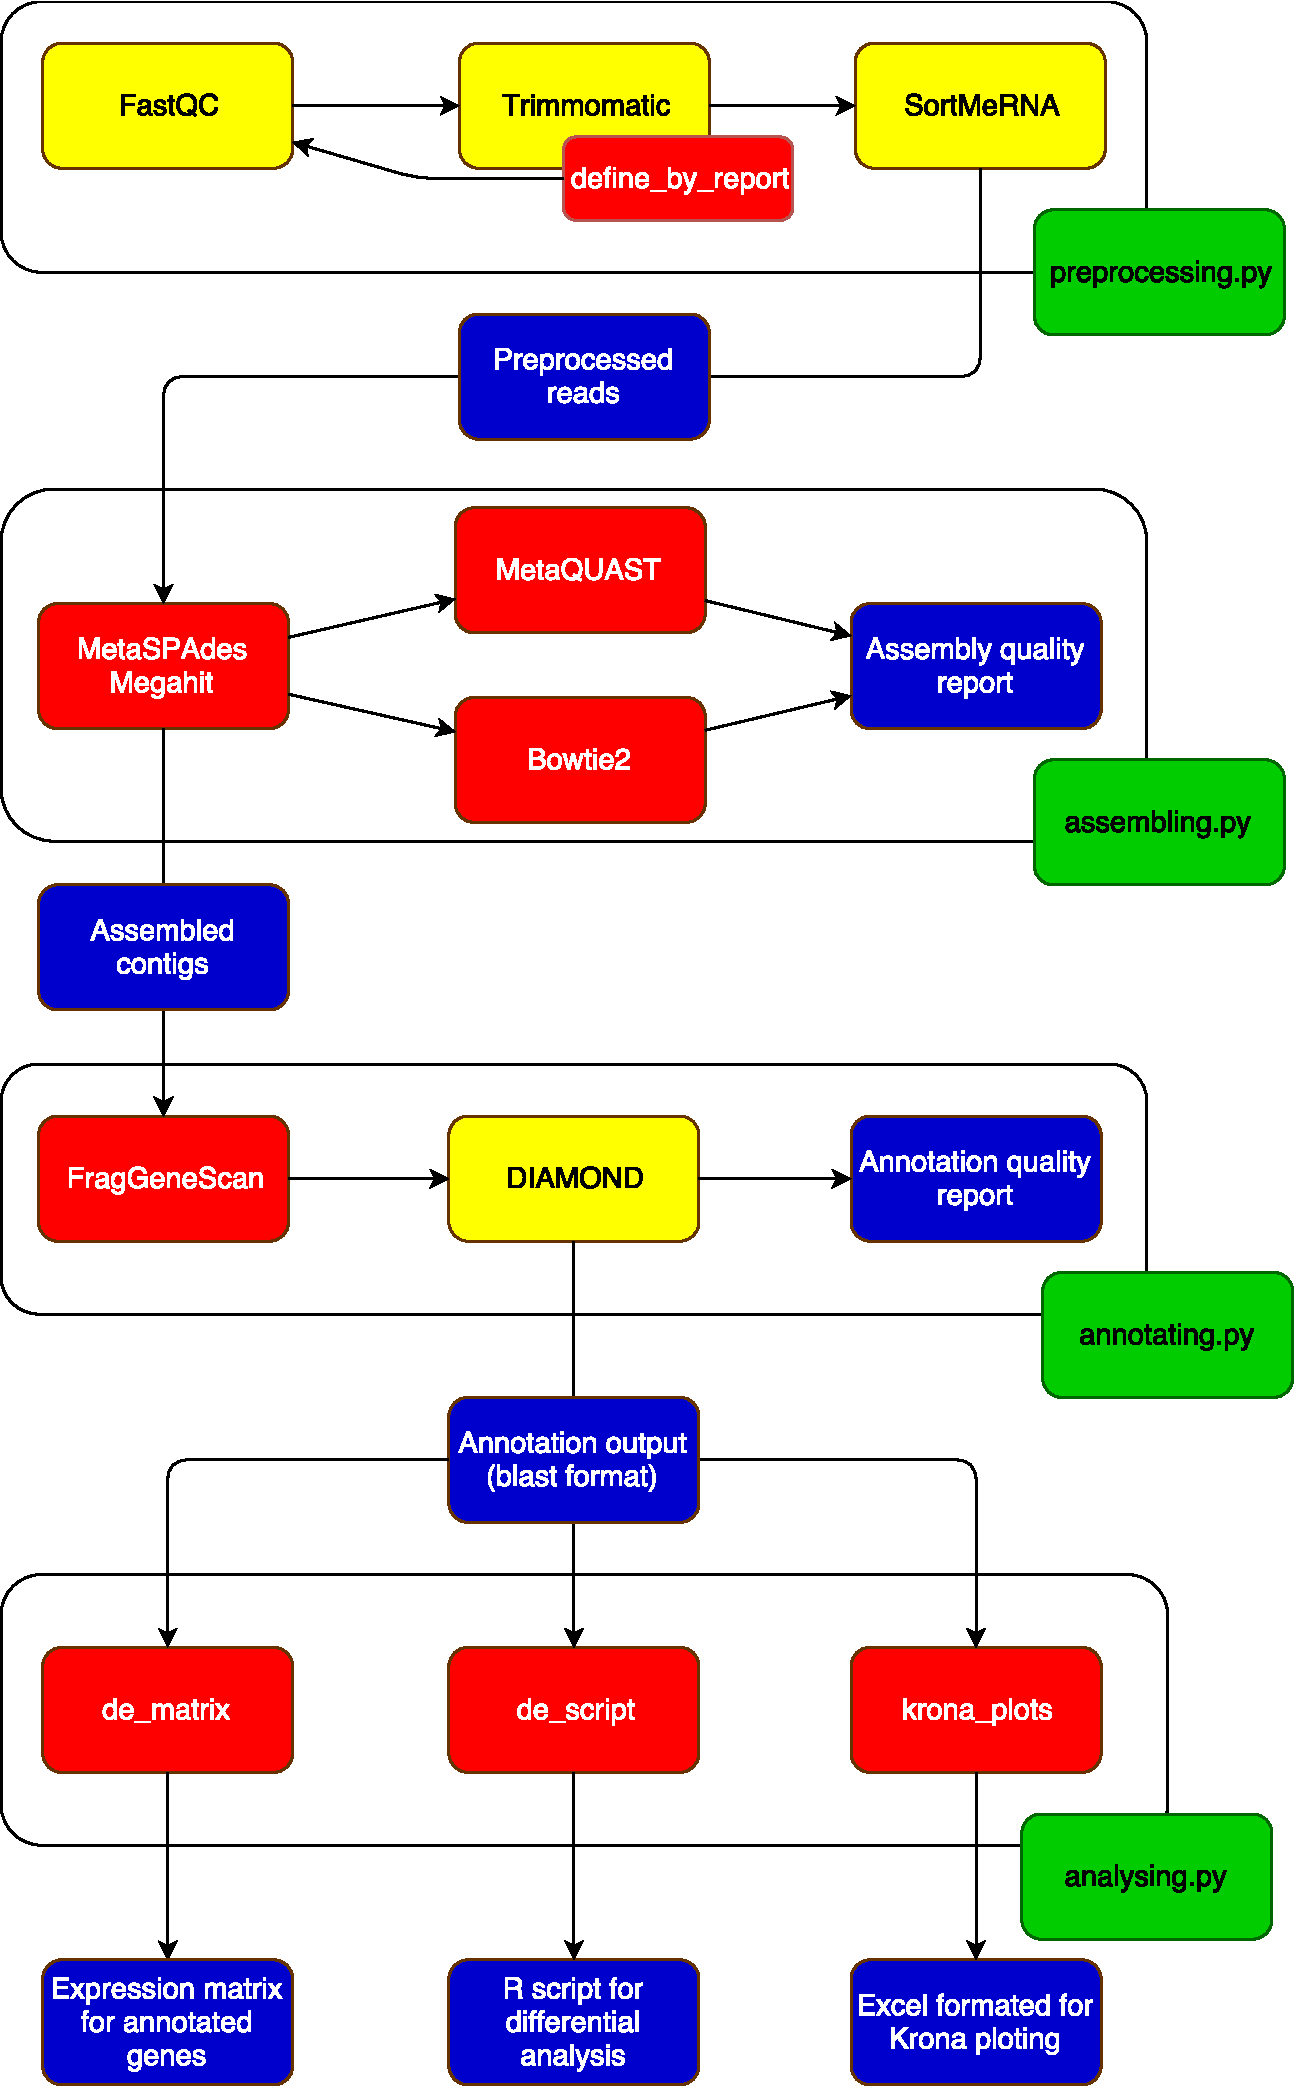
\includegraphics[width=\columnwidth,height=\textheight]{FiguresUndTables/Development/mosca_classes.pdf}
    \caption{The four scripts (green) integrating the four steps of meta-omics analysis, by incorporating wrappers for some tools in the form of classes (yellow) and functions (red). Some of the functions integrate additional functionalities, like the ones present in the analysis phase. Output files (blue) connect the various steps of the pipeline.}
    \label{fig:moscaclasses}
    \end{figure}
    
    The preprocessing of \gls{mosca} includes the following steps:
    \begin{enumerate}
        \item Quality control of raw \gls{ngs} data by running FastQC (version 0.11.4) - provides information about the quality of the reads, and allows the identification of adapters and bias during sequencing;
        
        \item Adapters removal - supplying the right file of adapters, Trimmomatic (version 0.32) excels at removing adapter presence in the data, with its "ILLUMINACLIP" tool. If the data was obtained by Illumina sequencing the adapter files can be obtained together with the Trimmomatic distribution available in GitHub \footnote{https://github.com/timflutre/trimmomatic}. \gls{mosca} will automatically search for adapter sequences in the data, identify which Illumina adapters were used and then remove them from the data. The presence of adapters results in the detection of overrepresented sequences by FastQC. After the adapter removal step, those overrepresented sequences corresponding to the adapters should disappear;
        
        \item Low quality sequences removal - \gls{mosca} reads the FastQC report obtained after the adapters removal step and solves the problems related to the "warning" and "fail" flags associated with bad data, by using several tools available in the Trimmomatic toolbox;
        
        \item Removal of \gls{rrna} - \gls{rrna} sequences are filtered by SortMeRNA (version 2.0) using SILVA database as the reference database;
        
        \item Quality assessment post-preprocessing – after all preprocessing steps, reads are again submitted to FastQC quality check. Ideally, the final FastQC report should not have any warning or failed flags.
    \end{enumerate}
    
    A general script calls all the classes that compose the collection of wrappers for these four tools (FastQC, Trimmomatic and SortMeRNA) and the additional functions to Trimmomatic, namely the determination of adapters with ILLUMINACLIP and FastQC and the quality trimming adusted in the arguments for CROP and HEADCROP with reference to the FastQC report.
    
    The preprocessing.py script makes use of the classes developed as wrappers of FastQC, Trimmomatic and SortMeRNA for the preprocessing steps (figure \ref{fig:moscaclasses}). Here, the data with a different nature namely, files containing \gls{mg}, \gls{mt} or 16S \gls{rrna} gene data are distinctively manipulated in some steps. It also distinguishes between single- or paired-end reads (all data manipulation tools integrated in \gls{mosca} support single- and paired-end modes).
    
    FastQC provides a report in tabular and visual (HTML) formats, with information concerning several aspects of \gls{ngs} data quality, divided in several analysis modules: Basic statistics, Per base sequence quality, Per tile sequence quality, Per sequence quality scores, Per base sequence content, Per sequence GC content, Per base N content, Sequence length distribution, Sequence duplication levels, Overrepresented sequences, Adapter content and Kmer content.
    
    For each analysis module a flag is given, meaning that the result is entirely normal (green), slightly abnormal (yellow) or very unusual (red), concerning the degree of deviation from an excellent report.
    
    FastQC results are used to define the parameters for adapter removal and quality trimming with Trimmomatic. In the adapter removal phase, FastQC\'s tabular report is parsed, and analyzed - if overrepresented sequences are detected, and are related to adapters, ILLUMINACLIP will be tested with all the adapter files. The adapter files used will be those that have "PE" in the name in the case of a \gls{pe} analysis, or "SE" in the case of a \gls{se} analysis. After each ILLUMINACLIP trimming, a FastQC report will be generated over the resulting file, and if the file no longer has adapter presence, then it will be used for the next steps. ILLUMINACLIP is used with values of 2, 30 and 10 for seed mismatches, palindrome clip threshold and simple clip threshold, respectively. The adapter files are downloaded from Trimmomatic's github project \footnote{https://github.com/timflutre/trimmomatic/tree/master/adapters}, if no adapter files are available. All this is implemented through the function "remove\_adapters".
    
    Trimmomatic is a toolkit packed with several functionalities for \gls{ngs} data trimming, designed specifically to work with Illumina reads. Five of its tools are implemented in \gls{mosca}:
    
    \begin{enumerate}
        \item ILLUMINACLIP - Trimmomatic distribution contains several Illumina files (Table \ref{adapter_files}) containing the platform's artificial sequences that can be formed during the sequencing workflow. These artificial sequences files can be assessed through the Trimmomatic’s GitHub project \footnote{https://github.com/timflutre/trimmomatic} and have not been updated since 2015. However, \gls{mosca} will ask if the user wants to check for updated files, and if so it will automatically download the files from the given location.
        \item HEADCROP – The FastQC module "Per Base Sequence Content" gives the proportion of each base position. In a random library, little differences between the different bases (A, T, G and C) are expected and, thus, the different lines obtained should be as parallel as possible. If not, it means there is an abnormal presence of a certain nucleotide at a certain position in the data. Usually, abnormal situations occur at the beginning of the sequences, and so HEADCROP will remove those first bases at the beginning, to the point where the difference between A, T, G and C is lower than 10\% . there is no longer a significant bias towards any nucleotide.
        \item CROP - Sequencing quality usually decreases at the end of the reads. \gls{mosca} uses the CROP tool to remove all the nucleotides from the position where the quality of the reads falls below a certain threshold (lower quartile below 10 or median less than 25), based on the "Per Base Sequence Quality" module results from the FastQC report. 
        \item AVGQUAL - in an effort to increase the robustness of preprocessing \gls{ngs} datasets, a minimum average quality is imposed, so only sequences above a defined threshold follow the next steps of analysis
        \item MINLEN - \gls{mosca} keeps reads with a minimum read length of 100 nucleotides. Reads with less than 100 nucleotides are removed using the MINLEN tool from Trimmomatic.
    \end{enumerate}
    
    The six files with Illumina artificial sequences were considered for the preprocessing \ref{adapter_files}. This sequences are available from Trimmomatic distribution.
    
    \begin{table}[]
    \centering
    \caption{The six artificial sequences files available from Trimmomatic distribution, two for \gls{se} and four for \gls{pe} mode, and the corresponding sequencing kits from Illumina.  The TruSeq3-PE-2.fa file contains the same sequences as the TruSeq3-PE.fa, but containing their reverse complements, it allows for palindrome clipping.}
    \label{adapter_files}
    \begin{tabular}{ll}
    \hline
    Adapter files available              & Sequencing technology            \\ \hline
    NexteraPE-PE                         & Nextera \gls{dna} kits                 \\
    TruSeq2-SE, TruSeq2-PE               & TruSeq RNA Library Prep Kit v2   \\
    TruSeq3-SE, TruSeq3-PE, TruSeq3-PE-2 & TruSeq PE Cluster Kit v3-cBot-HS \\ \hline
    \end{tabular}
    \end{table}
    
    After adapter removal by ILLUMINACLIP, \gls{mosca} calls the function "define\_by\_report", making use of several different Trimmomatic\'s tools for different quality trimming tasks. With CROP, \gls{mosca} removes the bases of all reads from the position after which the average quality in that position falls below the defined threshold for a warning flag in the FastQC report - if, in the boxplot representing the quality distribution in that position, the lower quartile falls below 10 or the median is less than 25. With HEADCROP, \gls{mosca} removes bases until the last position at which there is a significant difference in the quantity of certain bases (if the difference between A and T or G and C is over 10\%). \gls{mosca} removes reads with an average quality under 20 (using AVGQUAL), and finally removes all sequences with less than 100 nucleotides in length (using "MINLEN"). Because every FastQC report is related to one file, even when handling paired-end data, \gls{mosca} will use Trimmomatic in single-end mode for cropping the less desirable extremities of the reads, but will not remove any read, as to conserve the paired-end nature of the data. When removing reads with the AVGQUAL tool, it will again use Trimmomatic in paired-end mode.
    
    SortMeRNA is used with the SILVA database, separating the sequences aligned to the database from the sequences not aligned. Because SortMeRNA accepts only one input file at a time, when working in paired-end mode two bash scripts \footnote{https://github.com/biocore/sortmerna/tree/master/scripts} must be used, one for merging the two files into one with interlaced reads, and the other to separate the reads into two files, after \gls{rrna} removal. Paired-in and paired-out arguments must be used to specify to SortMeRNA that the input file is paired-end data. The non aligned reads file is used for the next steps.
    
    \subsection{Assembly}
    
    \gls{mosca} allows to choose between two assemblers, MetaSPAdes (version 3.9.0) and Megahit (version 1.1.1). They were chosen because of their superior performance in previous studies, and because even though they are similar tools, they implement several distinctive solutions to problems inherent to assembly. Megahit, for example, employs "succint de Bruijn graphs" to reduce memory requirements and discards singleton k-mers, while also implementing "mercy-k-mer" strategy, thus obtaining more relevant data, while MetaSPAdes uses complete read information together with preassembled reads at every step of its workflow, and in contrast to most assemblers, it directly incorporates paired end information in the graphs by building it with k-bimers, instead of using ofter construction of the Bruijn graph for simplification steps \citep{Vollmers2017}. 
    
    In their default mode, MetaSPAdes and Megahit iterate through several kmers for the same assembling procedure, generating several contig files, from which the most reliable contigs are chosen. Even though they both support reference-based assembling, for now \gls{mosca} only operates on \textit{de novo} assembling, since it aims to analyze data collected from complex microbial communities containing several unknown microorganisms without complete genomic information available.
    
    After the assembly, MetaQUAST (version 4.5) is used as a tool for quality control of the assembly. It produces reports for several classical metrics on the final contigs, like N50, number of contigs for several sizes, and number of misassemblies. Bowtie2 (version 2.2.6) is also used to complete the assembly report by giving the percentage of preprocessed reads that can be aligned to the obtained contigs, i.e., the percentage of reads used in the assembly.
    
    The assembling.py script takes into account the existence of two options for assembler - MetaSPAdes and Megahit -, generating the commands for both tools, and integrating MetaQUAST and Bowtie2 for posterior check on the quality of the assembly, returning a final report with the analysis performed by these two  tools (Figure \ref{fig:moscaclasses}).
    
    Both MetaSPAdes and Megahit run as default to make a multi-kmer assembly: 
    \begin{enumerate}
        \item MetaSPAdes iterates over k-mer sizes 21, 33 and 51, and outputs several files for every k-mer and for the more reliable contigs,:
        \begin{enumerate}
            \item The contigs in FASTA format (contigs.fasta)
            \item The scaffolds (scaffolds.fasta)
            \item The assembly graph (assembly\_graphp.fastg)
            \item The scaffold paths in the assembly graph (scaffolds.paths)
            \item The contigs before read resolution (before\_rr.fasta)
        \end{enumerate}
        \item Megahit iterates through the k-mer values 21, 29, 39, 59, 79, 99, 119 and 141, and besides the final contigs file, for each contig value it outputs five files:
        \begin{enumerate}
            \item The contigs in FASTA format (.contigs.fa)
            \item The contigs with local low coverage \textit{unitigs} removed (.addi.fa)
            \item The locally assembled contigs for that specific kmer (.local.fa)
            \item The stand-alone contigs for that specific kmer (.final.contigs.fa)
            \item A file related with bubble representation of contigs (.bubble\_seq.fa)
        \end{enumerate}
    \end{enumerate}
    
    \gls{mosca} uses the final contigs files (i.e., contigs.fa or contigs.fasta) for posterior analysis obtained from the default set of parameters. These files are used as input for generating the quality report.
    
    The quality control is based on the report from MetaQUAST, with one final line added from the alignment of Bowtie2. MetaQUAST and Bowtie2 together report for a number of metrics in \gls{mosca}:
    \begin{enumerate}
        \item Number of contigs, total and for several intervals (over 10000\gls{bp}, for example)
        \item Duplication ratio - total number of bases aligned to the assembly divided by the total number of aligned bases in the reference genome
        \item Genome fraction (\%) - percentage of aligned bases in the reference genome
        \item N50, N75, L50 and L75
        \item Reads aligned (\%)
    \end{enumerate}
    
    \subsection{Annotation}
    
    In \gls{mosca}, FragGeneScan (version 1.15) is used for gene calling in the annotation step.
    
    A function was developed to build the FragGeneScan command and perform gene calling, with the contigs files (.fa file from Megahit or .fasta file from Metaspades) as input. Because the contigs were used instead of reads, the arguments were set as following: complete as "1" and train as "complete". 
    
    FragGeneScan outputs three files:
    \begin{enumerate}
        \item The list of the coordinates of putative genes (.out)
        \item A FASTA of nucleotide sequences corresponding to the putative genes (.ffn)
        \item A FASTA of aminoacid sequences corresponding to the putative genes (.fna)
    \end{enumerate}
    
    DIAMOND (version 0.9.9) is used to align the assembled contigs with the sequences present in reference databases in FASTA format, and is run in default conditions. It was chosen because it is much faster than the existing alternatives, such as BLAST. \gls{mosca} determines the number of \gls{orf}s identified and the number of \gls{orf}s that could be annotated by using the selected FASTA database. 
    
    \gls{mosca} uses the FragGeneScan aminoacid sequences file as input for DIAMOND. DIAMOND uses "blastp" for the identification of aminoacid sequences, and requires a database (.dmnd) as input for aligning the sequences. Compressed or uncompressed FASTA databases can be converted to .dmnd format with the "makeblastdb" tool from DIAMOND. 
    
    Blastp may output several alignments for each of the sequences, from the most to the less confident, and MOSCA only considers the best hit, with the smaller e-value. The annotated reads are then outputed in a .blast file, and the unaligned reads in a .fasta file.
    
    \subsection{Data analysis} 
    
    \gls{mosca} integrates UniProt's database in its workflow, allowing to use UniProt's ID mapping service for obtaining relevant data in specific formats: a tab-separated report with taxonomic (superkingdom, phylum, class, order, family, genus and species) and systems (EC number,  pathways and protein names) information, and the GFF file with information about the features present in the sequences. Because UniProt has a maximum limit of 2Mb of information for submission, the list of IDs must be broken into chunks, and one chunk must be submitted at a time. This taxonomy and functional information is used to create CSV files formatted for generating Krona plots.
    
    For \gls{mt} experiments, \gls{mosca} produces an expression matrix from the values of coverage of the annotated genes, and generates a script for \gls{de} using DeSEQ2 (version 1.18.1). Heatmaps are generated giving information on the degree of similarity between samples, and on the differential gene expression.
    
    The analysing.py script receives as input the blast result from DIAMOND (aligned.blast file), and converts it into a pandas DataFrame object, for which it has integrated three functionalities (Figure \ref{fig:moscaclasses}): 
    \begin{enumerate}
        \item krona\_plots - If the annotation was performed with reference to the UniProt database, \gls{mosca} will use the \gls{api} provided by UniProt to retrieve relevant taxonomic and systems information and output it as CSVs. Quantification of annotated \gls{orf}s for each taxonomic and systems category determines the area for the Krona plots.
        \item de\_matrix - For \gls{mt} studies, de\_matrix builds an expression matrix from the coverage values calculated by the assemblers, and retrieves the sequences IDs from DIAMOND's report, thus building a matrix that is outputted for the \gls{de} analysis in R. The values on this matrix are normalized by \gls{tpm}.
        \item de\_script - For \gls{mt} studies, de\_script builds the R script for \gls{de} analysis with DESeq2, to be used over the built matrix.
    \end{enumerate}
    
    The \gls{tpm} normalization that takes place in the build up of the \gls{de} matrix follows three steps:
    \begin{enumerate}
        \item For each annotated gene, the coverage value is divided by the length of the corresponding gene, in the length column of DIAMOND's report. This gives \gls{rpk}.
        \item The sum of all \gls{rpk} values in the sample is calculated, and divided by 1000000. This is the "per million" scaling factor.
        \item The \gls{rpk} values are divided by the "per million" scaling factor, giving \gls{tpm}.
    \end{enumerate}
    
    This analysis outputs two types of graphics:
    \begin{enumerate}
        \item From the taxonomic and systems information, two CSV files are outputted in a format that can be used directly for krona ploting, using pandas \textit{convert\_to\_csv} function.
        \item From the R package DeSEQ2, heatmaps are outputed concerning multisample similarity comparison and \gls{de} of the most significantly expressed genes.
    \end{enumerate}
    
    \subsection{Implementation details}
    
    \gls{mosca} was developed in python 3.6.0, and tested in a Ubuntu xenial 16.04.2 desktop version.
    The source code of \gls{mosca} and more information concerning the pipeline can be found on github \footnote{https://github.com/iquasere/MOSCA}.

    The following libraries have been used in the development for distinct purposes.
    
    \paragraph{subprocess}
    
    Implements command line functionality through python scripting, used for the input/output workflows between the several tools integrated \footnote{https://docs.python.org/2/library/subprocess.html}. In \gls{mosca}, usually the command is first generated as a string, in the form that it would be inserted in the command line, and then subprocess runs the command.
    
    \paragraph{pandas}
    
    Implements data structures and analysis \footnote{http://pandas.pydata.org}. In \gls{mosca}, it is used for storing the result of parsing FastQC's and DIAMOND's reports and UniProt's information files into DataFrames.
    
    \paragraph{Requests}
    
    A python library for performing HTTP requests \footnote{http://docs.python-requests.org}. Used for performing the HTTP request steps in the analysis of results from annotation.
    
    \chapter{Pipeline testing}
    
    \section{Datasets for pipeline testing}
	
	\gls{mosca} was tested with real datasets obtained from lab scale anaerobic digestion bioreactors. For \gls{mg}/\gls{mt}, the data was retrieved from four continuous bioreactors inoculated with the same inoculumtreating synthetic wastewater containing ethanol or a mixture of volatile fatty acids. The main goals were to identify the pathways most utilized and the most active microorganisms and compare these functional and taxonomic information obtained from the different operational conditions. In this work, the \gls{mg} samples from this study were named "DNA1", "DNA2", "DNA3" and "DNA4", while the corresponding \gls{mt} samples were named "RNA1", "RNA2", "RNA3" and "RNA4".

	For \gls{mg}/\gls{mp}, the data was extracted from anaerobic batch reactors converting different \gls{lcfa} to methane. In this work, only the \gls{mg} samples, named "DNA5", "DNA6", "DNA7" and "DNA8", were tested with MOSCA. 

	Three datasets retrieved from amplicon sequencing experiments targeting the 16S \gls{rrna} gene, also obtained from anaerobic bioreactors, were used, as well, for testing some of the tools implemented in \gls{mosca}. These samples were designated by "RRNA1", "RRNA2" and "RRNA3".
	
	All FastQ files were obtained in \gls{pe} format, and so all the tools used until the assembly, inclusively, were used in \gls{pe} format. \gls{pe} sequencing produces two different files per sample, one named "forward" and the other "reverse", since one has the sequences from the forward strand and the other the ones from the reverse strand.
	
	\section{Results}
    
    \subsection{Preprocessing}
    
    \subsubsection{Initial data quality assessment}
    
    Before testing the artificial sequences removal capacity of ILLUMINACLIP, eight metagenomic FastQ files (DNA1 to DNA8) were submitted to FastQC evaluation.
    
    It was possible to obtain high quality FastQ files at the end of the trimming with Trimmomatic as it is shown in table \ref{fig:trim_mg}. All the original files presented "warn" or "fail" based on FASTQC analysis for overrepresented sequences. In general, after the first step of trimming, the ILLUMINACLIP, the adapters were removed and the warnings resolved. Per base sequence quality (PBSQ) passed the quality check only after the trimming based on FASTQC report (that gives the information on the quality of the sequences). This trimming step used the CROP tool to remove the bases at the end of the sequences that presented low quality. 
    These results were obtained by setting the following parameters: 
    \begin{enumerate}
        \item ILLUMINACLIP - seed mismatches of 2, palindrome clip threshold of 30 and simple clip threshold of 10
        \item AVGQUAL - minimum quality of 20
        \item MAXINFO - target length of 40, strictness of 0.5
    \end{enumerate}
    
    The ILLUMINACLIP was capable, when using the right adapter file, of removing completely the presence of overrepresented sequences, and even reducing "fail" and "warn" flags in the Kmer Content to smoother reports, showing that those irregularities were associated with the presence of artificial sequences in the datasets.
    
    \begin{table}[ph!]    
    \caption{Quality evaluation results \tnote{*}  using FastQC on \gls{mg} FastQ files (DNA1 to DNA8) before and after trimming with Trimmomatic. Green color means "pass", yellow color means "warn" and red color means "fail".}
    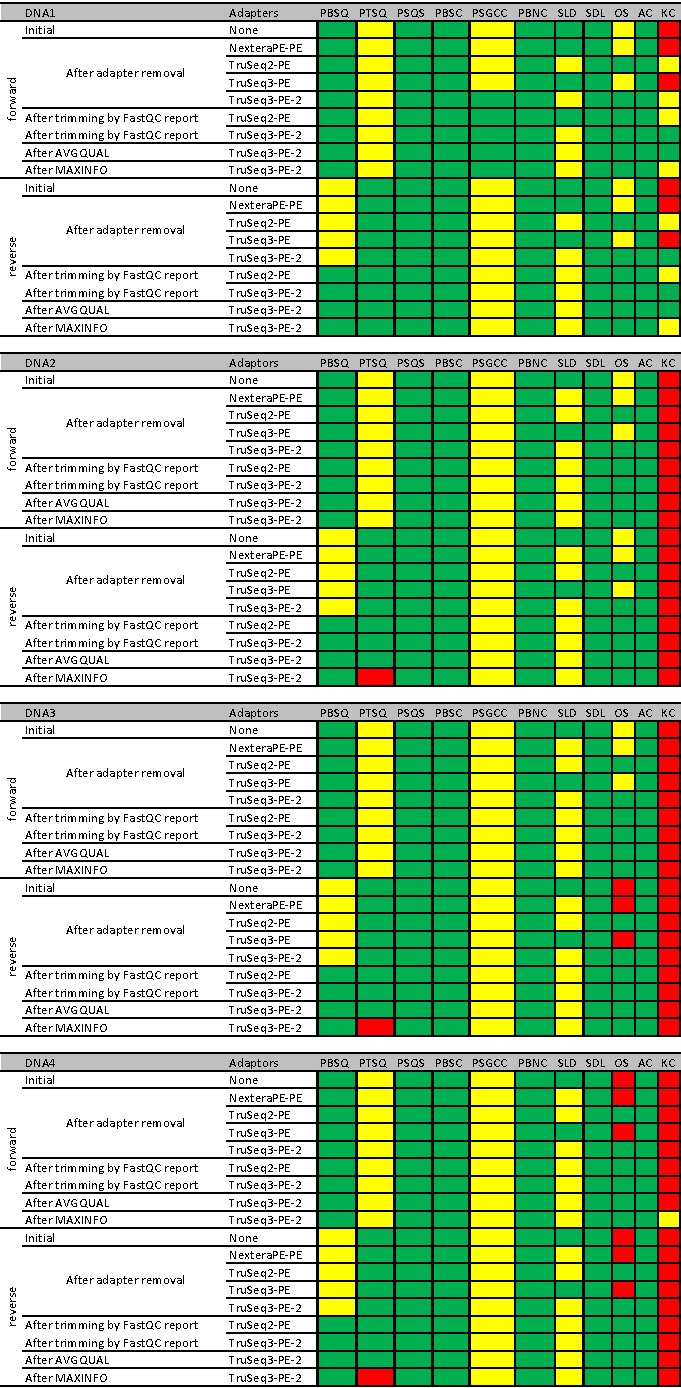
\includegraphics[width=\columnwidth,height=\textheight]{FiguresUndTables/Results/Preprocessing/fastqcdna1234.pdf}
    \label{fig:trim_mg}
    \begin{tablenotes}
    \item[*] \tiny PBSQ: Per Base Sequence Quality; PTSQ: Per Tile Sequence Quality; PSQS: Per Sequence Quality Scores; PBSC: Per Base Sequence Content (PBSC); PSGCC: Per Sequence GC Content; PBNC: Per Base N Content; SLD: Sequence Length Distribution; SDL: Sequence Duplication Levels; OS: Overrepresented Sequences; AC: Adapter Content; KC: Kmer Content.
    \end{tablenotes}
    \end{table}
    
    \begin{table}[ph!] \ContinuedFloat
    \caption{Continued.}
    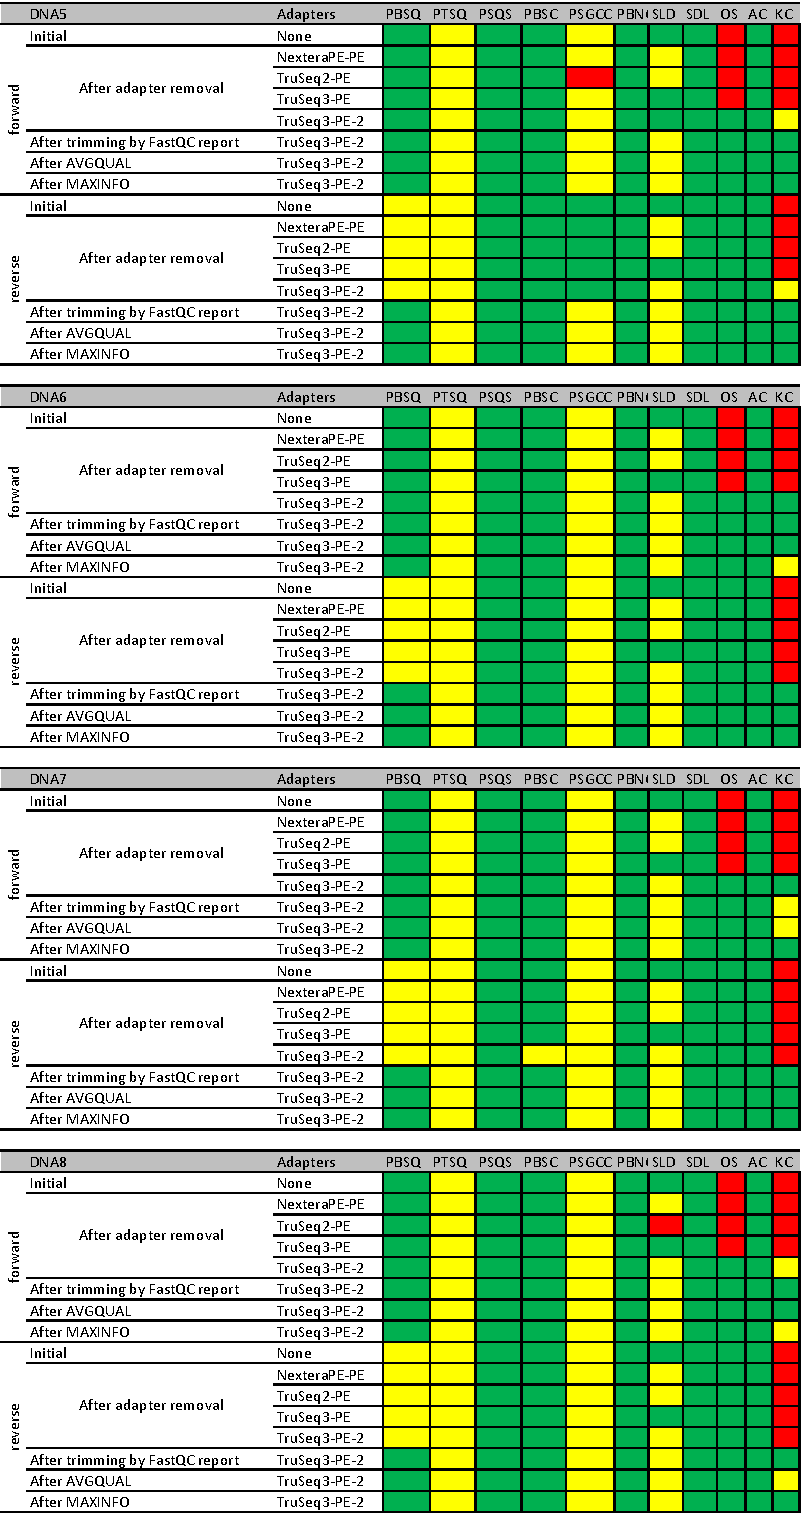
\includegraphics[width=\columnwidth,height=\textheight]{FiguresUndTables/Results/Preprocessing/fastqcdna5678.pdf}
    \end{table}

    FastQ files obtained from 16S metagenomics showed much different reports, due to the different nature of the data. "Per base sequence content", "Overrepresented sequences" and "Sequence Duplication Levels" all reported severe bias, but these biases were due to the conserved nature of \gls{rrna} and to the fact that these files were obtained from amplicon sequencing targeting the 16S \gls{rrna} gene (table \ref{fig:trim_16s}).
    
    \begin{table}[ph!]    
    \caption{Quality evaluation results using FastQC on metagenomics 16S rRNA genes FastQ files (RRNA 1 to 3) before and after trimming with Trimmomatic. Green color means "pass", yellow color means "warn" and red color means "fail".}
    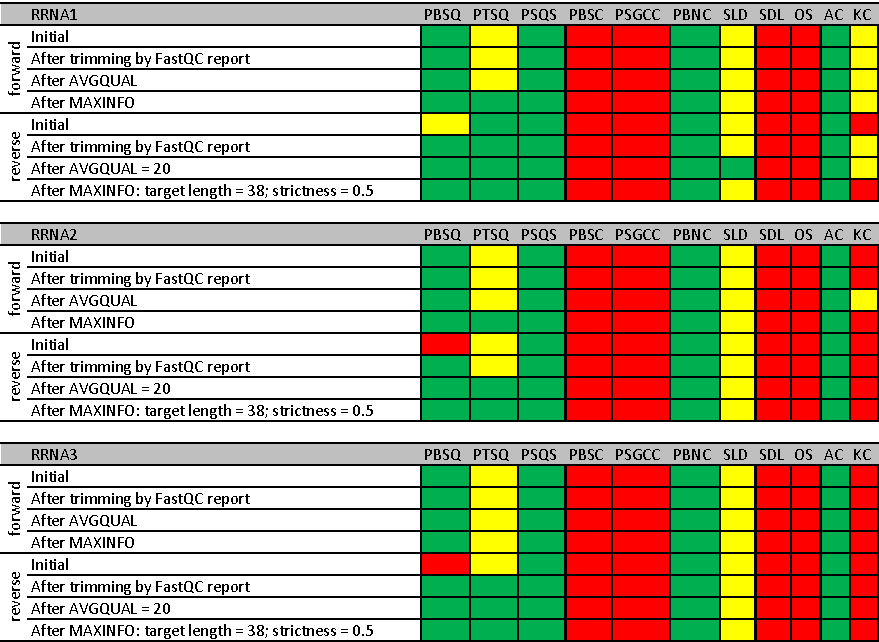
\includegraphics[width=\columnwidth,height=\textheight/2]{FiguresUndTables/Results/Preprocessing/fastqcrrna.pdf}
    \label{fig:trim_16s}
    \end{table}
    
    \subsubsection{Trimming by FastQC report}
    
    In the case of \gls{mg} data (DNA1 to DNA8), for all reverse files, a warning was issued by FastQC concerning the general quality of the reads towards the last positions, in a per position report, and towards the first positions, when considering relative nucleotide abundance. After using the CROP tool adjusted to the first position from which the quality is under the defined threshold and using the HEADCROP tool for the position after which there is a normal relative abundance of each nucleotide, \gls{mosca} was capable of improving the quality of the data, since this two simple steps solved the irregularities reported by FastQC on the corresponding modules (Table \ref{fig:trim_mg} and \ref{fig:trim_16s}).
    
    In the analysis of 16S \gls{rrna} files no sequences were identified as artificial by FastQC, so ILLUMINACLIP was not used. FastQC reported a strong bias at several positions of the data, which is justified by the conserved nature of 16S sequences. Therefore, the HEADCROP functionality was not used for the trimming, but because of decline in quality at the end of sequences, CROP was used, with results similar to those of DNA samples.
    
    \subsubsection{rRNA removal by SortMeRNA}
    
    \begin{table}[ph!]    
    \caption{Number of reads in the datasets throughout preprocessing, number of contigs after assembly, number of \gls{orf}s identified in the contigs and number of genes annotated with reference to the UniProt database.}
    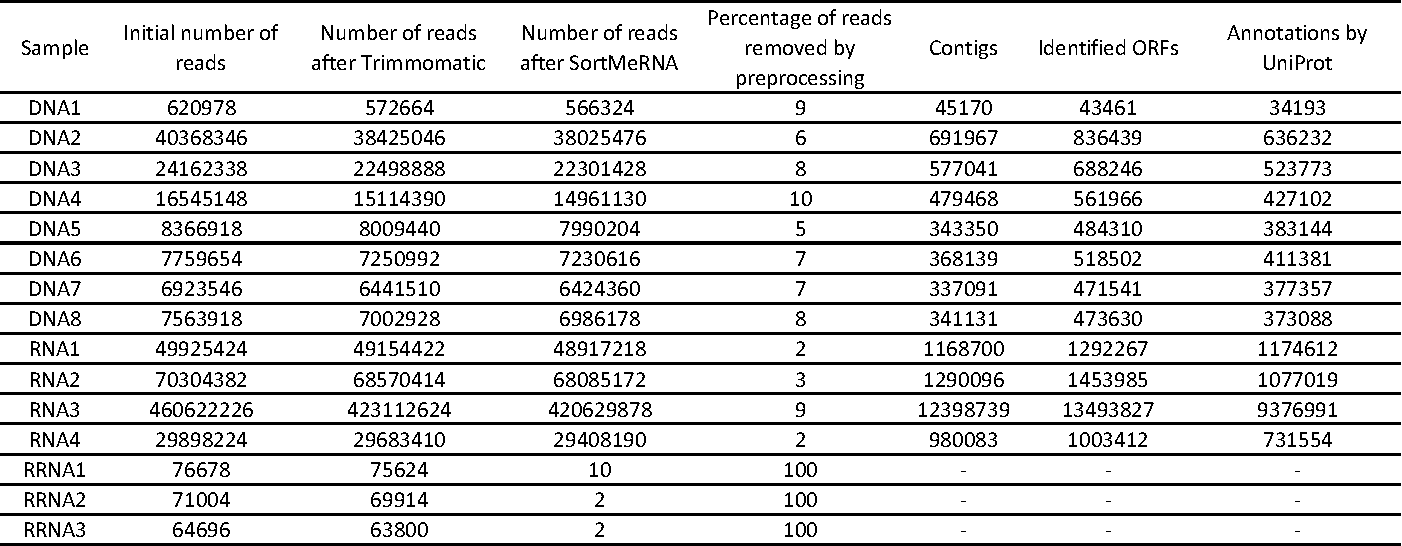
\includegraphics[width=\columnwidth]{FiguresUndTables/Results/numbers.pdf}
    \label{fig:preprocessing_general}
    \end{table}
    
    \gls{rrna} sequences were aligned to those present in SILVA and RFAM databases in order to detect and remove the 16S \gls{rrna} sequences by using Sortmerna (Table \ref{fig:preprocessing_general}). Two different kinds of dataset were tested: three samples, forward and reverse, of \gls{rrna} amplicon sequencing, where ideally it would be expected total identification of reads as \gls{rrna}; eight samples of \gls{dna} /\gls{mg} and four of \gls{rna} (\gls{mt}), with forward and reverse information, where only a low percentage should be identified as \gls{rrna}. SortMeRNA was very efficient in identifying the \gls{rrna} from the 16S samples, with 99.99\% of sequences identified as \gls{rrna}. Less than 1\% of the reads were removed, on average, from the DNA samples (Table \ref{fig:preprocessing_general}), thus proving the sensibility and specificity of SortMeRNA.
    
    \subsection{Assembly}
        
    MEGAHIT and MetaSPAdes were run using the predefined/default arguments (see section 3.1.2), and both used a multi-kmer approach for assembling the \gls{mg} reads. The percentage of reads used for the assembly was estimated, by using Bowtie2 to align the original reads with the contigs produced, and several metrics were calculated by MetaQUAST (Tables \ref{fig:assembling_quality} and \ref{fig:assembling_quality1}).
    
    At least 70\% of reads were aligned with Bowtie2 to the contigs, with the exception of DNA1, which may be related with the small size of the dataset, when compared to the others. With MetaSPAdes, the results were even better, with more reads aligned, more contigs assembled and higher N50s. For this reason, MetaSPAdes contigs were used in the next steps.
    
    \begin{table}[ph!]
    \caption{Several metrics concerning the quality of the contigs produced by MEGAHIT, obtained by MetaQUAST and Bowtie2.}
    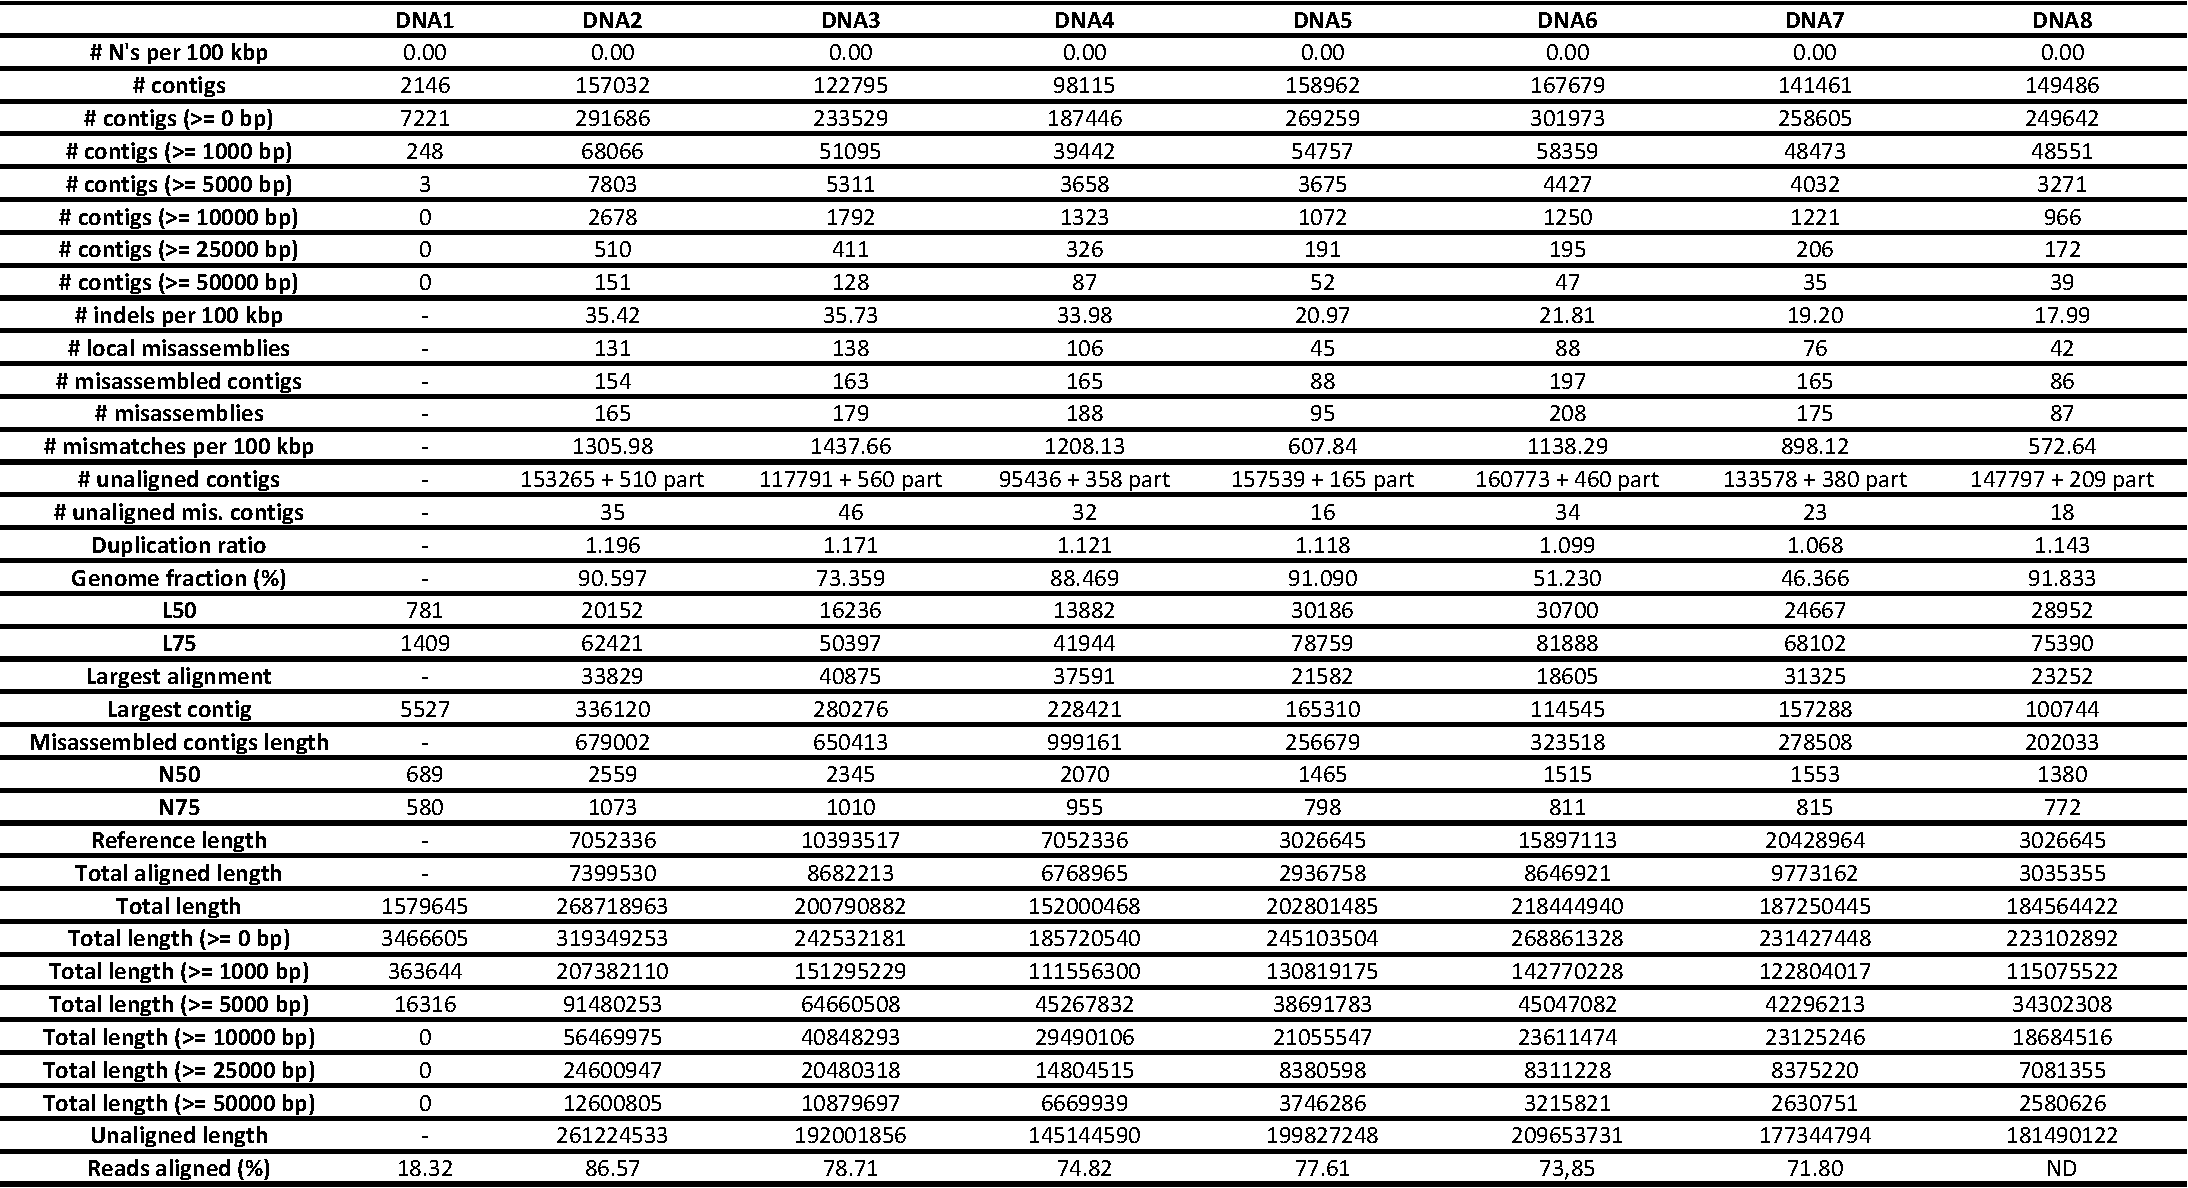
\includegraphics[width=\columnwidth]{FiguresUndTables/Results/Assembling/assembly_results.pdf}
    \label{fig:assembling_quality}
    \end{table}
    
    \begin{table}[ph!]
    \caption{Several metrics concerning the quality of the contigs produced by MetaSPAdes, obtained by MetaQUAST and Bowtie2.}
    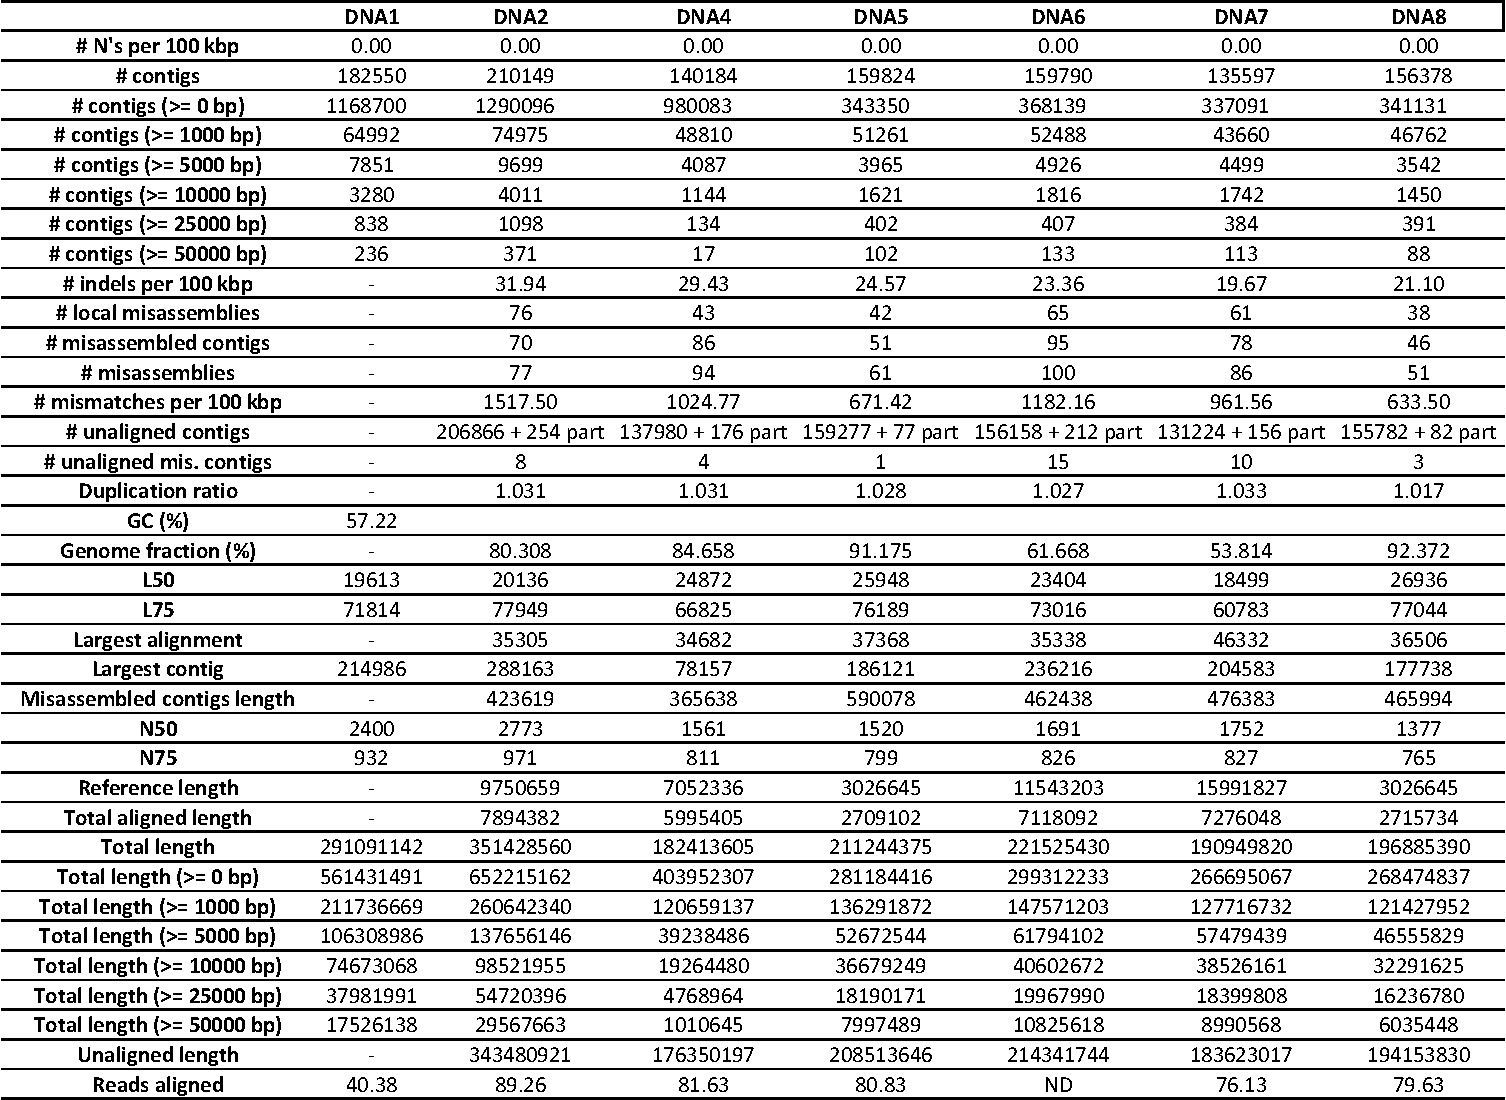
\includegraphics[width=\columnwidth]{FiguresUndTables/Results/Assembling/assembly_results1.pdf}
    \label{fig:assembling_quality1}
    \end{table}

    \subsection{Annotation}
    
    FragGeneScan was used to detect the \gls{orf}s in the contigs generated by MetaSPAdes. DIAMOND was used to align the \gls{orf}s identified by FragGeneScan to sequences in the UniProt database. Approximately 78\% of the identified \gls{orf}s could be annotated by aligning to UniProt. For each read, only the most confident alignment was considered, and for each alignment, the following information was retrieved: the ID of the sequence that the \gls{orf} aligned to, the percentage of identity between the \gls{orf} and the sequence it aligned to, the length of the sequence from UniProt, the number of mismatch between the two sequences, the number of gap openings in the alignment, the first and last position of the \gls{orf} and of the sequence it aligned to, the e-value and the score of the alignment.
    
    \subsection{Data analysis}
    
    The UniProt ids were retrieved from the alignment files produced by DIAMOND, and submitted to the UniProt mapping service. Taxonomic and systems information was obtained, and the presence of the different taxa and subsystems was quantified, and represented in Krona plots (figures \ref{fig:krona_dna2tax} and \ref{fig:krona_dna2sys}, respectively).
    
    \begin{figure}[ph!]    
    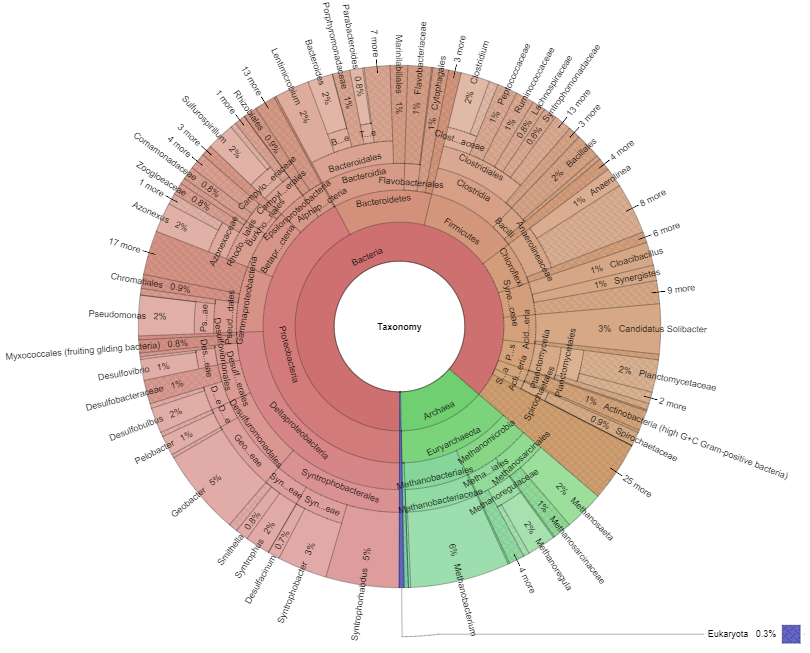
\includegraphics[width=\columnwidth]{FiguresUndTables/Results/Annotating/krona_dna2tax.png}
    \caption{Taxonomic identification of the species present in sample DNA2.}
    \label{fig:krona_dna2tax}
    \end{figure}
    
    \begin{figure}[ph!]    
    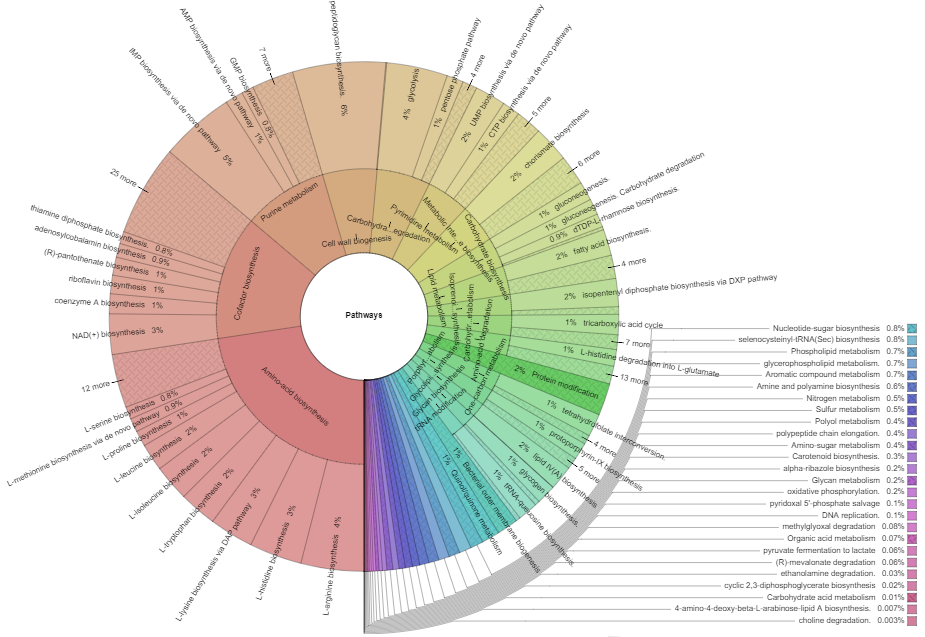
\includegraphics[width=\columnwidth]{FiguresUndTables/Results/Annotating/krona_dna2sys.png}
    \caption{Assignment of genes to pathways for the DNA2 sample.}
    \label{fig:krona_dna2sys}
    \end{figure}
    
    \gls{de} analysis was performed for three samples of \gls{rna}. Based on the coverage values obtained from assembling, a matrix was built, integrating information about every annotated gene in the assembled contigs. The values of that matrix were normalized with \gls{tpm} \citep{conesa2016survey}. \gls{de} analysis was performed in R using DeSEQ2 package and heatmaps were obtained for most differentially expressed genes (Figure \ref{fig:mainexpression}) and for denoting the differences between samples (Figure \ref{fig:sampledist}).
    
    \begin{figure}[!h]    
    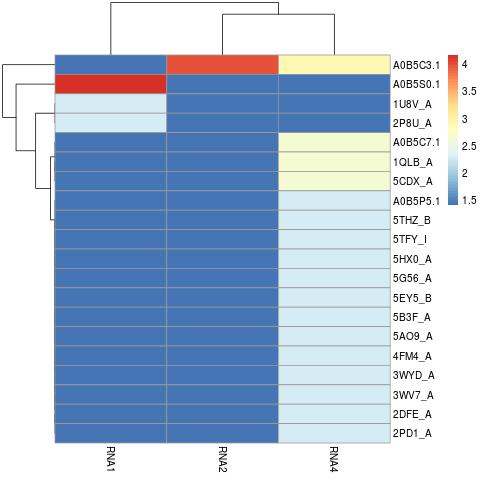
\includegraphics[width=\columnwidth]{FiguresUndTables/Results/Analyzing/mainexpression.jpg}
    \caption{Example of heatmap representing the most expressed genes in the three samples (RNA1, RNA2 and RNA4), and evidencing the differences in expression of the genes by a colour gradient.}
    \label{fig:mainexpression}
    \end{figure}
    
    \begin{figure}[!h]    
    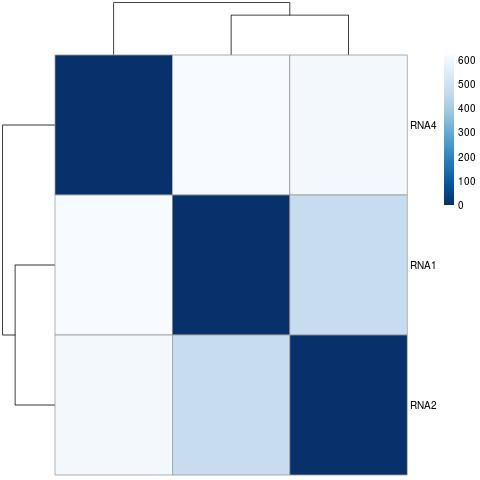
\includegraphics[width=\columnwidth]{FiguresUndTables/Results/Analyzing/sampledist.jpg}
    \caption{Example of heatmap denoting the distance between the three samples (RNA1, RNA2 and RNA4), illustrated in a colour gradient, with clustering of the distance values.}
    \label{fig:sampledist}
    \end{figure}
    
    \chapter{Conclusion}
    
    \gls{mosca} was developed as a Python command line tool for full automation of \gls{mg} and \gls{mt} data analysis. \gls{mosca} starts by applying successfully several pre-processing steps to raw input reads, then assemblies the reads into contigs and annotates the resulting sequences into taxonomic and biosystems information. For every main step there is a quality report, either obtained through custom scripts inside \gls{mosca} or through the functionalities already present in other tools. 
    
    A major improvement is that \gls{mosca} adapts the datasets trimming by adjusting Trimmomatic's arguments based on FastQC's reports. For \gls{mt} experiments, after the annotation step, \gls{mosca} builds a normalized matrix and generates a script that allows for \gls{de} analysis in R, thus allowing for multi-sample comparison of transcriptomes. \gls{mosca} is, therefore, the third tool to integrate \gls{mg} and \gls{mt} analysis, after \gls{imp} and \gls{fmap}.
    
    The results obtained are promising but there is space for several improvements. In the future, \gls{mosca} can be easily expanded to include \gls{mp} and/or \gls{mm} data analysis as well. Also, having a \gls{gui} would be useful to turn this automated pipeline into a more user friendly tool for integrated meta-omics data analysis. Even though \gls{mosca} is developed to maximize automation, more user input could allow for human augmented data analysis - VizBin is a good example, where the user handles the data in an interactively, visual way, for binning the contigs into subsets.
    
    %part not included
    \begin{comment}
    \subsection{Integration of metagenomic with metatranscriptomic data}
    
    \gls{mg} and \gls{mt} require similar software. For the preprocessing steps, the workflow of \gls{imp} seems stronger than that of \gls{fmap}, with less house built tools - quality control of reads is done with \textit{FASTQC}, removal of low quality and human (when justified) sequences with \textit{Trimmomatic}, gls{rrna} depletion (when justified) with \textit{SortMeRNA}. 
    
    For assembly, the \textit{de novo} co-assembly of \gls{imp} is a very interesting choice, making the most of \gls{mg} and \gls{mt} data in the assembly - therefore the integration of \textit{MEGAHIT} and \textit{IDBA-UD} seems a logical step.
    
    After the assembly, \textit{VizBin} may be used for binning the contigs, \textit{MetaQUAST} to verify the quality of the process and BEDTools for calculating depth of coverage. After such analysis, \textit{Prokka} and \textit{MetaQUAST} could be implemented for functional and taxonomic annotation, respectively, of the contigs assembled \textit{de novo}.
    
    For the final analysis, integrating \textit{KronaTools} will allow the visualization of the results. Mapping of \gls{kegg} pathways will be provided as well and \textit{ShotgunFunctionalizeR} will allow for differential quantification of gene expression in one or between several samples.
    
    \subsection{Integration of metagenomic with metaproteomic data}
    
    The MPA workflow will be the basis for the development of the metaproteomics part of the pipeline. Including the four search engines \textit{X!Tandem}, \textit{OMSSA}, \textit{Crux}, \textit{Inspect}, plus the \textit{Mascot} software for the interpretation of \gls{ms} spectra will produce more protein annotations, validated with the overlap of the search engines' results. But since a \gls{mp} study deals with many unknown proteins, a \textit{de novo} assembler should be used, such as PepNovo \citep{frank2005pepnovo}, PEAKS \citep{ma2003peaks} or SEQUIT \citep{demine2004sequit}, to increase protein identification from microorganisms whose genomic information is not in databases. If \gls{mg} data is available it will be used to construct the protein database for protein identification. Annotation and results analysis will be performed similarly to what was described for \gls{mg} and \gls{mt} analysis.
    \end{comment}
    
    
	%- Bibliography (needs bibtex) -%
	\bibliography{library}

	% Index of terms (needs  makeindex) -------------
	%\printindex
	
	% APPENDIX --------------------------------------
	
	% Back Cover -------------------------------------------
	\umbackcover{}

\end{document}
